%!TEX root = ../thesis.tex
%*******************************************************************************
%*********************************** First Chapter *****************************
%*******************************************************************************

\chapter{Variant discovery in genome graphs}
\label{chap:denovo}
\ifpdf
    \graphicspath{{Chapter1/Figs/Raster/}{Chapter1/Figs/PDF/}{Chapter1/Figs/}}
\else
    \graphicspath{{Chapter1/Figs/Vector/}{Chapter1/Figs/}}
\fi
% ==================================================================
\setcounter{section}{-1}
\section{Publication and collaboration acknowledgements}
\label{sec:denovo-acknowledge}

The software program that this chapter extends, \pandora{}, was first conceived and implemented in Rachel Colquhoun's DPhil thesis \cite{rachelthesis}.

A paper describing \pandora{} and the work in this chapter is available at \cite{pandora}. This paper was a collaborative project that spans five years of work by Rachel (first author), myself (second author), Leandro Ishi (third author), and others.

My aim here is to clarify what work is solely mine and what was completed in collaboration. Where possible, I have also attempted to indicate within certain sections the work not completed by myself.

The method for performing \denovo{} variant discovery in \autoref{sec:denovo-method} is my own, with input from collaborators. However, I implemented it within the \pandora{} codebase. \autoref{sec:denovo-prune} describes a process for pruning the path-space in a de Bruijn graph, this work was the joint idea of myself and Leandro Ishi, and Leandro added the implementation for the distance map calculation.

All of the work in \autoref{sec:denovo-sims} is my own.

\autoref{sec:denovo-empirical} describes a subset of the results in \cite{pandora}. The evaluation framework used in the paper (and this section) underwent many iterations over two years. Leandro Ishi and I conceived and implemented the original method of calculating precision and recall in a coordinate-agnostic manner with the mapping of variant probes. This framework was later incorporated and adapted by Martin Hunt in the tool Varifier (\url{https://github.com/iqbal-lab-org/varifier}). Leandro Ishi implemented the final evaluation method but it is heavily based on the original work we performed together.

In addition, several components of the pipeline to run the analysis in \autoref{sec:denovo-empirical} and \cite{pandora} were initially implemented by myself but were later refactored or changed by Leandro.

The idea for the \ont{} basecalling model comparison in \autoref{sec:denovo-methylation} was mine, as was the initial implementation - but not the final. \autoref{sec:pandora-roc-results} was ultimately performed by Leandro Ishi; however, I had much input and contributed pipeline code in the beginning.

The construction of the pan-genome truth set of variants discussed in \autoref{sec:denovo-empirical-eval} and \autoref{app:pangenome-snp-truth} is the work of Leandro Ishi. It is included in this chapter to aid the reader's understanding of how recall is calculated.

% ==================================================================
\section{Introduction}

Standard approaches to variant analysis are effectively a first-order approximation. In such an approximation, samples are considered identical to a selected reference; one aligns sequencing reads to it, identifying apparent variations via the read pileup, and then the reference is modified to get an estimate of the sample's genome. We term such a procedure a "linear" or "single-reference" approach. 

As mentioned in \autoref{sec:pandora-intro}, \pandora{} is a method developed by a previous PhD student in our lab, Rachel Colquhoun \cite{rachelthesis}. \pandora{} works on the principle of approximating a genome as a hierarchical mosaic. At a high level, \pandora{} represents a pan-genome as a mosaic of loci, while at the locus level, it is a mosaic of previously observed genomes. Loci in this context can represent any genomic unit desired; a gene, intergenic region, or a mobile genetic element - the method is agnostic. Sequences from many genomes in a population are collapsed into a graph structure (\autoref{sec:make_prg}) to form a locus population reference graph (\prg{}). All of the pan-genome's \prg{}s are collected into the high-level pan-genome reference graph (\panrg{}).

When given a set of Illumina or \ont{} sequencing reads, \pandora{} identifies which \panrg{} loci are present and infers a consensus sequence for each. This consensus is the maximum likelihood path through the respective \prg{} and is used as the first-order approximation for the sample.

While \pandora{} - before the work in this chapter - enables the comparison of genomes to a level of detail provided by no other tool, there is still a significant shortcoming: it cannot discover novel mutations. As such, before the work presented in this chapter, \pandora{} was effectively a genotyping tool. If a sample contains a variant not present in a \prg{}, the best \pandora{} can do is select the path closest to that variant. Therefore, we begin this chapter by describing a method for performing \denovo{} variant discovery in a genome graph and implement it in \pandora{} - turning \pandora{} into a two-stage approximation method.

We use a simulated genome and associated \ont{} dataset to show that without this discovery capability, \pandora{} cannot detect variants absent from a \prg{}. In addition, we explore the impact of various parameters on the \denovo{} discovery method and find read depth to have a vital influence.

Finally, we use an empirical dataset consisting of 20 diverse \ecoli{} samples to show that with our new variant discovery approach, \pandora{} has higher recall than all single-reference tools tested for both Illumina and \ont{} data. In addition, we identify methylation sites as a major source of our errors on \ont{} data and provide a solution for removing many of these errors. In the process of performing this analysis, we outline a coordinate-free method for evaluating variant caller precision and recall, facilitating the comparison of linear- and graph-based methods. 

% ==================================================================
\section{Methods}
\label{sec:denovo-method}

We define a method that extends \pandora{}, with a subcommand \vrb{discover}, to allow for the \denovo{} discovery of variants not present in a \prg{}. We implemented it within the \pandora{} codebase in the C++ programming language. 

\pandora{}, as implemented by Rachel Colquhoun (before this chapter), approximates a novel genome as a mosaic of prior genomes - the nearest path through the \panrg{}. In this chapter, we add two further steps: first, locating regions of the mosaic which were not supported by reads ("candidate regions"), and second, performing a particular type of local assembly in those regions.

The first step of \denovo{} variant discovery in genome graphs is finding the candidate regions that show evidence of dissimilarity from the sample's reads.

\subsection{Finding candidate regions}
\label{sec:denovo-candidate-regions}

The input required for finding candidate regions are a locus \prg{} (node), $n$, within the \pandora{} \panrg{}; the maximum likelihood path of $n$, as both sequence $mlp_n$ and (minimizer) \kmer{}s, $kmlp_n$; and a padding size, $w$, for the number of positions surrounding the candidate region to retrieve.

We define a candidate region, $r$, as an interval within $mlp_n$ where read depth (coverage) is less than a given threshold, for less than $m$ consecutive positions. $m$ acts to restrict the size of variants we can detect. If set too large, the following steps become much slower due to the combinatorial expansion of possible paths. We note that coverage is actually stored on $kmlp_n$, but is stored for the whole \kmer{}. We convert the coverage on $kmlp_n$ into per-position coverage on $mlp_n$ and use that to identify low-coverage segments as described.  

\subsection{Enumerating paths through candidate regions}
\label{sec:path-enum}

For all candidate regions, $r$, we construct a \dbg{} $G_r$ from the subsequences of the reads that overlap $r$, using the GATB library \cite{gatb2014}. 

We define $A_L$ and $A_R$ as sets of \kmer{}s to the left and right of $r$ in the maximum likelihood path, $mlp_n$. They are anchors to allow insertion of new sequences found by \denovo{} discovery into the \prg{}. Each set has a maximum size of $k$.

We abandon \denovo{} discovery if no pairwise combination of $A_L$ and $A_R$ exists in the \dbg{} $G_r$.

We use sets of \kmer{}s for $A_L$ and $A_R$, rather than a single anchor \kmer{}, to provide redundancy in the case where sequencing errors cause some anchors to not be in $G_r$. We define the start anchor \kmer{}, $a_L$, as the first (left-most) $a_L \in A_L \land a_L \in G_r$. Likewise, we define the end anchor \kmer{}, $a_R$, as the left-most $a_R \in A_R \land a_R \in G_r$.

Now that we have two anchor \kmer{}s, $a_L$ and $a_R$, our goal is to find all valid paths between these anchors in $G_r$.

To identify valid paths, we perform depth-first search (DFS) on $G_r$, beginning from $a_L$, to obtain a spanning tree, $T_r$. $p_r$ is defined as a path from the root node $a_L$ of $T_r$ and ending at node $a_R$, which fulfils the following two conditions: i) $p_r$ is shorter than the maximum allowed path length; ii) no more than $k$ nodes along $p_r$ have coverage $< (0.1 n_r e_r)$, where $e_r$ is the expected \kmer{} coverage for $r$ and $n_r$ is the number of iterations of path enumeration for $r$.

$V_r$ is the set of all $p_r$ satisfying these conditions. If $|V_r|$ is greater than a predefined threshold, $\eta$, $n_r$ is incremented by 1 and $V_r$ is repopulated. If $0.1n_r = 1.0$ then \denovo{} discovery is abandoned for $r$.

The second condition listed above, which relies on $n_r$ and $e_r$, has the effect of progressively increasing the amount of coverage we demand on a candidate path ($p_r$). In the first iteration, $n_r=1$ - i.e., we require the path to have 10\% of the expected read depth (coverage). If this yields too many paths ($|V_r|>\eta$), we restart and require all paths to have 20\% of the expected coverage. Finally, if we reach a stage where we require 100\% of the expected coverage but still have too many paths, we quit \denovo{} discovery for the candidate region.

\subsection{Pruning the path-space in a candidate region}
\label{sec:denovo-prune}

As \pandora{} operates on both accurate and error-prone sequencing reads, the number of valid paths in $G_r$ can be immense. In testing, we found that the path enumeration process can result in runtimes beyond seven days in some scenarios. The increased runtime is due to cycles occurring in $G_r$ and exploring paths that will never reach our required end anchor ($a_R$). 

In order to reduce the path-space within $G_r$, we prune paths based on multiple criteria. Critically, this pruning happens at each step of the graph walk (path enumeration; \autoref{sec:path-enum}).

In addition to $T_r$, obtained by performing DFS on $G_r$, we produce a distance map $D_r$ that results from running reversed breadth-first search (BFS) on $G_r$, beginning from the \emph{end} anchor ($a_R$). We say reversed BFS as we explore the \emph{predecessors} of each node, rather than the successors. $D_r$ is a binary search tree where each node in the tree represents a \kmer{} in $G_r$ that is reachable from $a_R$ via reversed BFS. Each node additionally has an integer that describes the shortest path from that node to $a_R$.

We use $D_r$ to prune the path-space as follows. As we walk the candidate path ($p_r$) in \autoref{sec:path-enum}, for each node (\kmer{}; $v$) in the \dbg{} $G_r$, starting at $a_L$, we lookup $v$ in $D_r$ to see if $a_R$ can be reached in a minimum of $i$ nodes, where $i$ is defined as the maximum allowed path length minus the number of nodes walked to reach $v$. If one of these conditions is not met, we abandon $p_r$. 

The advantage of this pruning strategy is that we never explore paths that will not reach our endpoint. Additionally, we will discard any path once we have made too many loops around a graph cycle.

\noindent
To illustrate the benefit of this pruning algorithm, we present an example in \autoref{fig:pruning}. This graph represents $G_r$ ($T_r$ more specifically, as only nodes reachable from $a_L$ are present), with the nodes representing \kmer{}s. The anchor \kmer{}s $a_L$ and $a_R$ are coloured red, and the numbers associated with each node represent the distance map $D_r$ - indicating the length of the shortest path to $a_R$ from that node. The lighter blue nodes and dashed edges indicate nodes that would cause us to abandon a path walk. For example, if we have stipulated a maximum allowed path length of 4, starting at $a_L$, whenever we reach a light blue node, the number of steps taken to reach that node, plus the length of the shortest path from that node to $a_R$, will always be greater than 4. Take the path $a_L \rightarrow B \rightarrow C \rightarrow E \rightarrow F$; we have taken four steps to reach this node, yet the shortest path to $a_R$ is 2, meaning, in the best-case scenario, $p_r$ would have length 6. In this way, we prevent needlessly walking the section of the graph $F \rightarrow G \rightarrow H \rightarrow I$. While this is a small example, in real graphs, the saving is potentially huge.


\begin{figure}
    \centering
    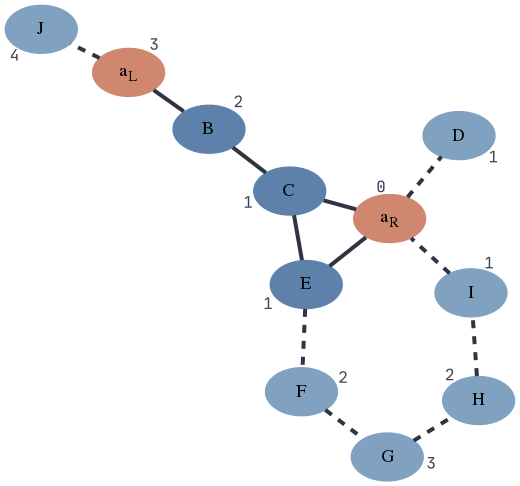
\includegraphics[width=0.7\textwidth]{Chapter1/Figs/pruning.png}
    \caption{An illustration of graph pruning. The graph represents a \dbg{} of a candidate region. Nodes represent \kmer{}s and are arbitrarily labelled, except $a_L$ and $a_R$ (red), which are the start and end anchor \kmer{}s, respectively. When enumerating paths, we aim to find all paths between $a_L$ and $a_R$ with a length no greater than a specified maximum. Numbers next to nodes indicate the length of the shortest path from that node to the end \kmer{} $a_R$. In this example, we set a maximum path length of 4. As such, light blue nodes and dashed edges indicate sections of the graph that would be pruned (not explored).}
    \label{fig:pruning}
\end{figure}

\hspace{0.75cm}

\noindent
In the end, for each candidate region ($r$), we are left with a collection of paths ($V_r$) between two \kmer{}s ($a_L$ and $a_R$). We create the final candidate paths by replacing the sequence between $a_L$ and $a_R$ in the maximum likelihood path ($mlp_n$) with each path ($p_r$) in $V_r$. These are written to file - with one file per candidate region. Padding the candidate paths in this way ensures they are inserted into the \prg{} in the correct location (see \autoref{sec:denovo-insert}). 


\subsection{Updating a \panrg{} with candidate paths}
\label{sec:denovo-insert}

As new paths may alter the structure of a \prg{}, we cannot insert them directly and must rebuild each \prg{} for which a candidate path is discovered.

The first step of rebuilding each locus \prg{} is to add the new candidate paths to the original multiple sequence alignment (MSA). We ensure the novel paths align with the correct section of the locus because we padded each candidate with the maximum likelihood path. Next, we combine all candidate paths for a locus into a single, unaligned FASTA file and add them to the existing locus MSA with the \vrb{--add} protocol in MAFFT \cite{katoh2012}. 

Finally, we run \makeprg{} on the subsequent alignments, and the resulting updated \prg{}s are combined into a single \panrg{} and indexed with \pandora{}. 

This updated \panrg{} can then be used as input to \pandora{}, and subsequent genotyping will include the novel variants.

% ==================================================================
\section{Initial assessment via simulations}
\label{sec:denovo-sims}
Having described an extension of the \pandora{} program that allows for \denovo{} variant discovery, we now perform an initial evaluation and explore the impact of various parameters using a simulated dataset.

\subsection{Methods}
\label{sec:denovo-sims-methods}

The first step in evaluating the effect of adding \denovo{} variant calling to \pandora{} is with a simulated dataset. We aim to show that the addition of \denovo{} discovery allows \pandora{} to improve its capacity for variant detection (recall) with minimal impact on the quality of the calls (precision). 

To construct our simulated dataset, we randomly select 100 gene MSAs from a pool of 29,702 obtained for \ecoli{} from the panX database \cite{panx}. Next, a \prg{} is constructed for each MSA with \makeprg{} (\autoref{sec:make_prg}). We used a range of \makeprg{} maximum nesting levels - 1, 3, 5, and 10 - to investigate whether \prg{} nesting has an impact on our ability to discover novel variants. The \prg{}s are combined into a single \panrg{} for each nesting level. A random path through each \prg{} is selected using \pandora{}, and these sequences are concatenated together to form a single "genome" sequence. 

We subsequently add SNPs to the simulated genome at different per-gene rates using \vrb{snp-mutator} \cite{snpmutator}. For this work, we introduce 100, 400, and 1,000 SNPs to the simulated genome, which equate to approximately 1, 4, and 10 SNPs per gene, respectively. \vrb{snp-mutator} produces a VCF of the SNPs that were introduced, along with the mutated genome sequence.

Next, we simulated 30,000 \ont{} reads from the mutated genomes using \vrb{nanosim-h} \cite{yang2017,brinda2018}. As the most recent model offered by \vrb{nanosim-h} was from the old R9 \ont{} flow cell, we trained and used a model from a freely-available \ecoli{} R9.4 dataset (\url{http://lab.loman.net/2017/03/09/ultrareads-for-nanopore/}). Each read set was randomly subsampled to a read depth (coverage) of 15, 30, 60, and 100 with \vrb{rasusa} \cite{rasusa2019} so we can investigate the impact of coverage on our ability to discover novel variants.

\pandora{}'s \vrb{discover} routine is then run, using the original panX-derived \panrg{} and the reads simulated from the mutated genome. Using this approach, we know that the reads originate from a sequence in our \panrg{}, but with some SNP differences and \ont{} errors. It is possible that some of the random SNPs introduced by \vrb{snp-mutator} already exist in the \panrg{}, but this is likely a minimal number. We use three different \kmer{} sizes for the \denovo{} discovery: 11, 13, and 15. 

After running the \vrb{discover} routine, we are left with a collection of candidate paths produced by the \denovo{} component. We then add these candidate paths back into the \panrg{} as per \autoref{sec:denovo-insert}. The updated \panrg{} is then used as input - along with the simulated reads - to \pandora{} \vrb{map} to produce a genotyped VCF that hopefully contains all of the simulated SNPs.

In parallel to this, we also run \pandora{} \vrb{map} on the original \panrg{} and simulated reads - i.e., without variant discovery. The genotyped VCF produced by this run shows how \pandora{} performed before the addition of \denovo{} variant discovery in this chapter. Theoretically, we only expect this VCF to contain simulated SNPs that were already in the \panrg{}.

At the end of this workflow, we have a genotyped VCF with and without \denovo{} variant discovery for each combination of maximum nesting, \denovo{} \kmer{} size, SNP rate, and read depth (coverage).

\subsection{Evaluation}
\label{sec:denovo-sims-eval}

Comparing the truth VCF to the one produced by \pandora{} requires care. The variants in the truth VCF are with respect to a linear reference genome; as we only simulated SNPs, these are single-position records. However, the \pandora{} variants are with respect to a graph and, depending on the density of variation in the graph, may not appear as single-position records (see \autoref{fig:min-match-len-example} for an illustration of this). 

We avoid the error-prone conversion of linear coordinates into graph coordinates, or vice versa, by using a coordinate-free evaluation. This approach maps variant \emph{probes} to each other and compares the probe sequences.  

We define a probe-set $P$ as a collection of probes, $p$, where $p$ represents an entry, $e$, in a VCF file, $V$. For each $e \in V$, $p$ is constructed by the concatenation of $l_w$, $e_c$, and $r_w$ (in that order), where $e_c$ is the called allele of $e$, and $l_w$ and $r_w$ are the sequences, of maximum length $w$, in the VCF reference to the left and right, respectively, of $e_c$. For \pandora{}, the VCF reference is the maximum likelihood sequence, and for the truth VCF it is the simulated genome (without the simulated SNPs).

A truth probe-set, $P_t$, was constructed from the VCF of variants added to the simulated genome and a query probe-set, $P_q$, from the variants called by \pandora{}. We then mapped all probes from $P_t$ to $P_q$ using \vrb{bwa mem} \cite{li2013}. We classify each probe in $P_t$ as a true positive (TP) if the $e_c$ part of the probe exactly matches the sequence it aligns to in $P_q$, or a false negative (FN) otherwise. Any probe in $P_q$ that does not have a TP truth probe mapped to it is classified as a false positive (FP). We perform this assessment for the "no \denovo{}" and "with \denovo{}" VCF files from \pandora{}. 

Precision is defined as the number of TPs divided by the number of TPs and FPs $precision=\frac{TP}{TP+FP}$; it represents the fraction of variant calls made that are correct. Likewise, recall is calculated as $recall=\frac{TP}{TP+FN}$ and describes the proportion of expected variants correctly discovered.

\subsection{Results}
\label{sec:denovo-sims-results}

We first look at \autoref{fig:denovo-sims}, which shows how precision and recall of the \pandora{} \denovo{} variants changes depending on the combination of parameters chosen. Those parameters were the read depth (coverage) of the simulated reads (\autoref{fig:denovo-sims-covg}), the number of SNPs introduced into the simulated genome (\autoref{fig:denovo-sims-num-snps}), the \kmer{} size used for variant discovery (\autoref{fig:denovo-sims-kmer-size}), and the maximum nesting level allowed in the \prg{}s (\autoref{fig:denovo-sims-nesting}). In total, there are 144 different combinations of parameters, and thus data points.

The parameter that appears to have the most visible impact on the precision and recall is the coverage (\autoref{fig:denovo-sims-covg}). It is somewhat unsurprising that as coverage increases, so do both precision and recall. However, there does not seem to be any noticeable difference for coverage $\ge 60$.

In the best case, the highest recall and precision values are 0.91 and 1.0, respectively. The data point is the same in both instances, with a coverage of 60, \kmer{} size of 13, number of SNPs 100, and a maximum nesting level of 10. Upon further investigation of the nine missed variants (FNs) for this data point, six were within $2k-1$ positions of the start or end of the locus, one was a null call (indicating genotyping uncertainty), one was falsely called as a homopolymer deletion, and the remaining missed call never had \denovo{} discovery triggered for that region of the locus. Therefore, only 3/9 FNs for this example (the last three) were discoverable with our \denovo{} method.

The last point requires some elaboration, as it may not be clear why only three FNs in the best-performing data point were expected to be detected by \denovo{}. As a reminder, the role of the \denovo{} component is to collect candidate alleles that are potentially in the sample but missing from the graph; if that set includes the truth, it has succeeded. Whether or not that true allele is genotyped as being present and recorded in the VCF is the job of the sequence inference and genotyping components of \pandora{}. In the case of the null genotype call, the correct variant was discovered, and it had higher coverage than the reference allele (26 vs 11); therefore, it is a failure of the genotyping. The homopolymer deletion is a failure of the genotyping; while \denovo{} (incorrectly) discovered the candidate indel, it also discovered the correct allele, but the genotyping chose the homopolymer deletion. Furthermore, the variant which \denovo{} discovery was never initiated for most likely has enough coverage on the reference allele that a candidate region was not detected - by default, we only flag a candidate region if coverage drops below 3.

In the case of the six missed calls near the ends of loci, these are not detectable by our current \denovo{} method as they occur within $2k-1$ positions of the boundary of a locus. The reason this makes them undetectable is related to our need for start and end anchor \kmer{}s in order to find candidate paths (\autoref{sec:path-enum}). The start and end \kmer{}s are a collection of $k$ \kmer{}s, meaning $2k-1$ positions are required surrounding a candidate region in order to be able to initiate \denovo{} discovery. We will return to this limitation later (\autoref{sec:fw-path-enum}).

\begin{figure}
     \centering
     \begin{subfigure}[b]{0.475\textwidth}
        \centering
        \caption[position=above]{Simulated coverage (read depth)}
        \label{fig:denovo-sims-covg}
        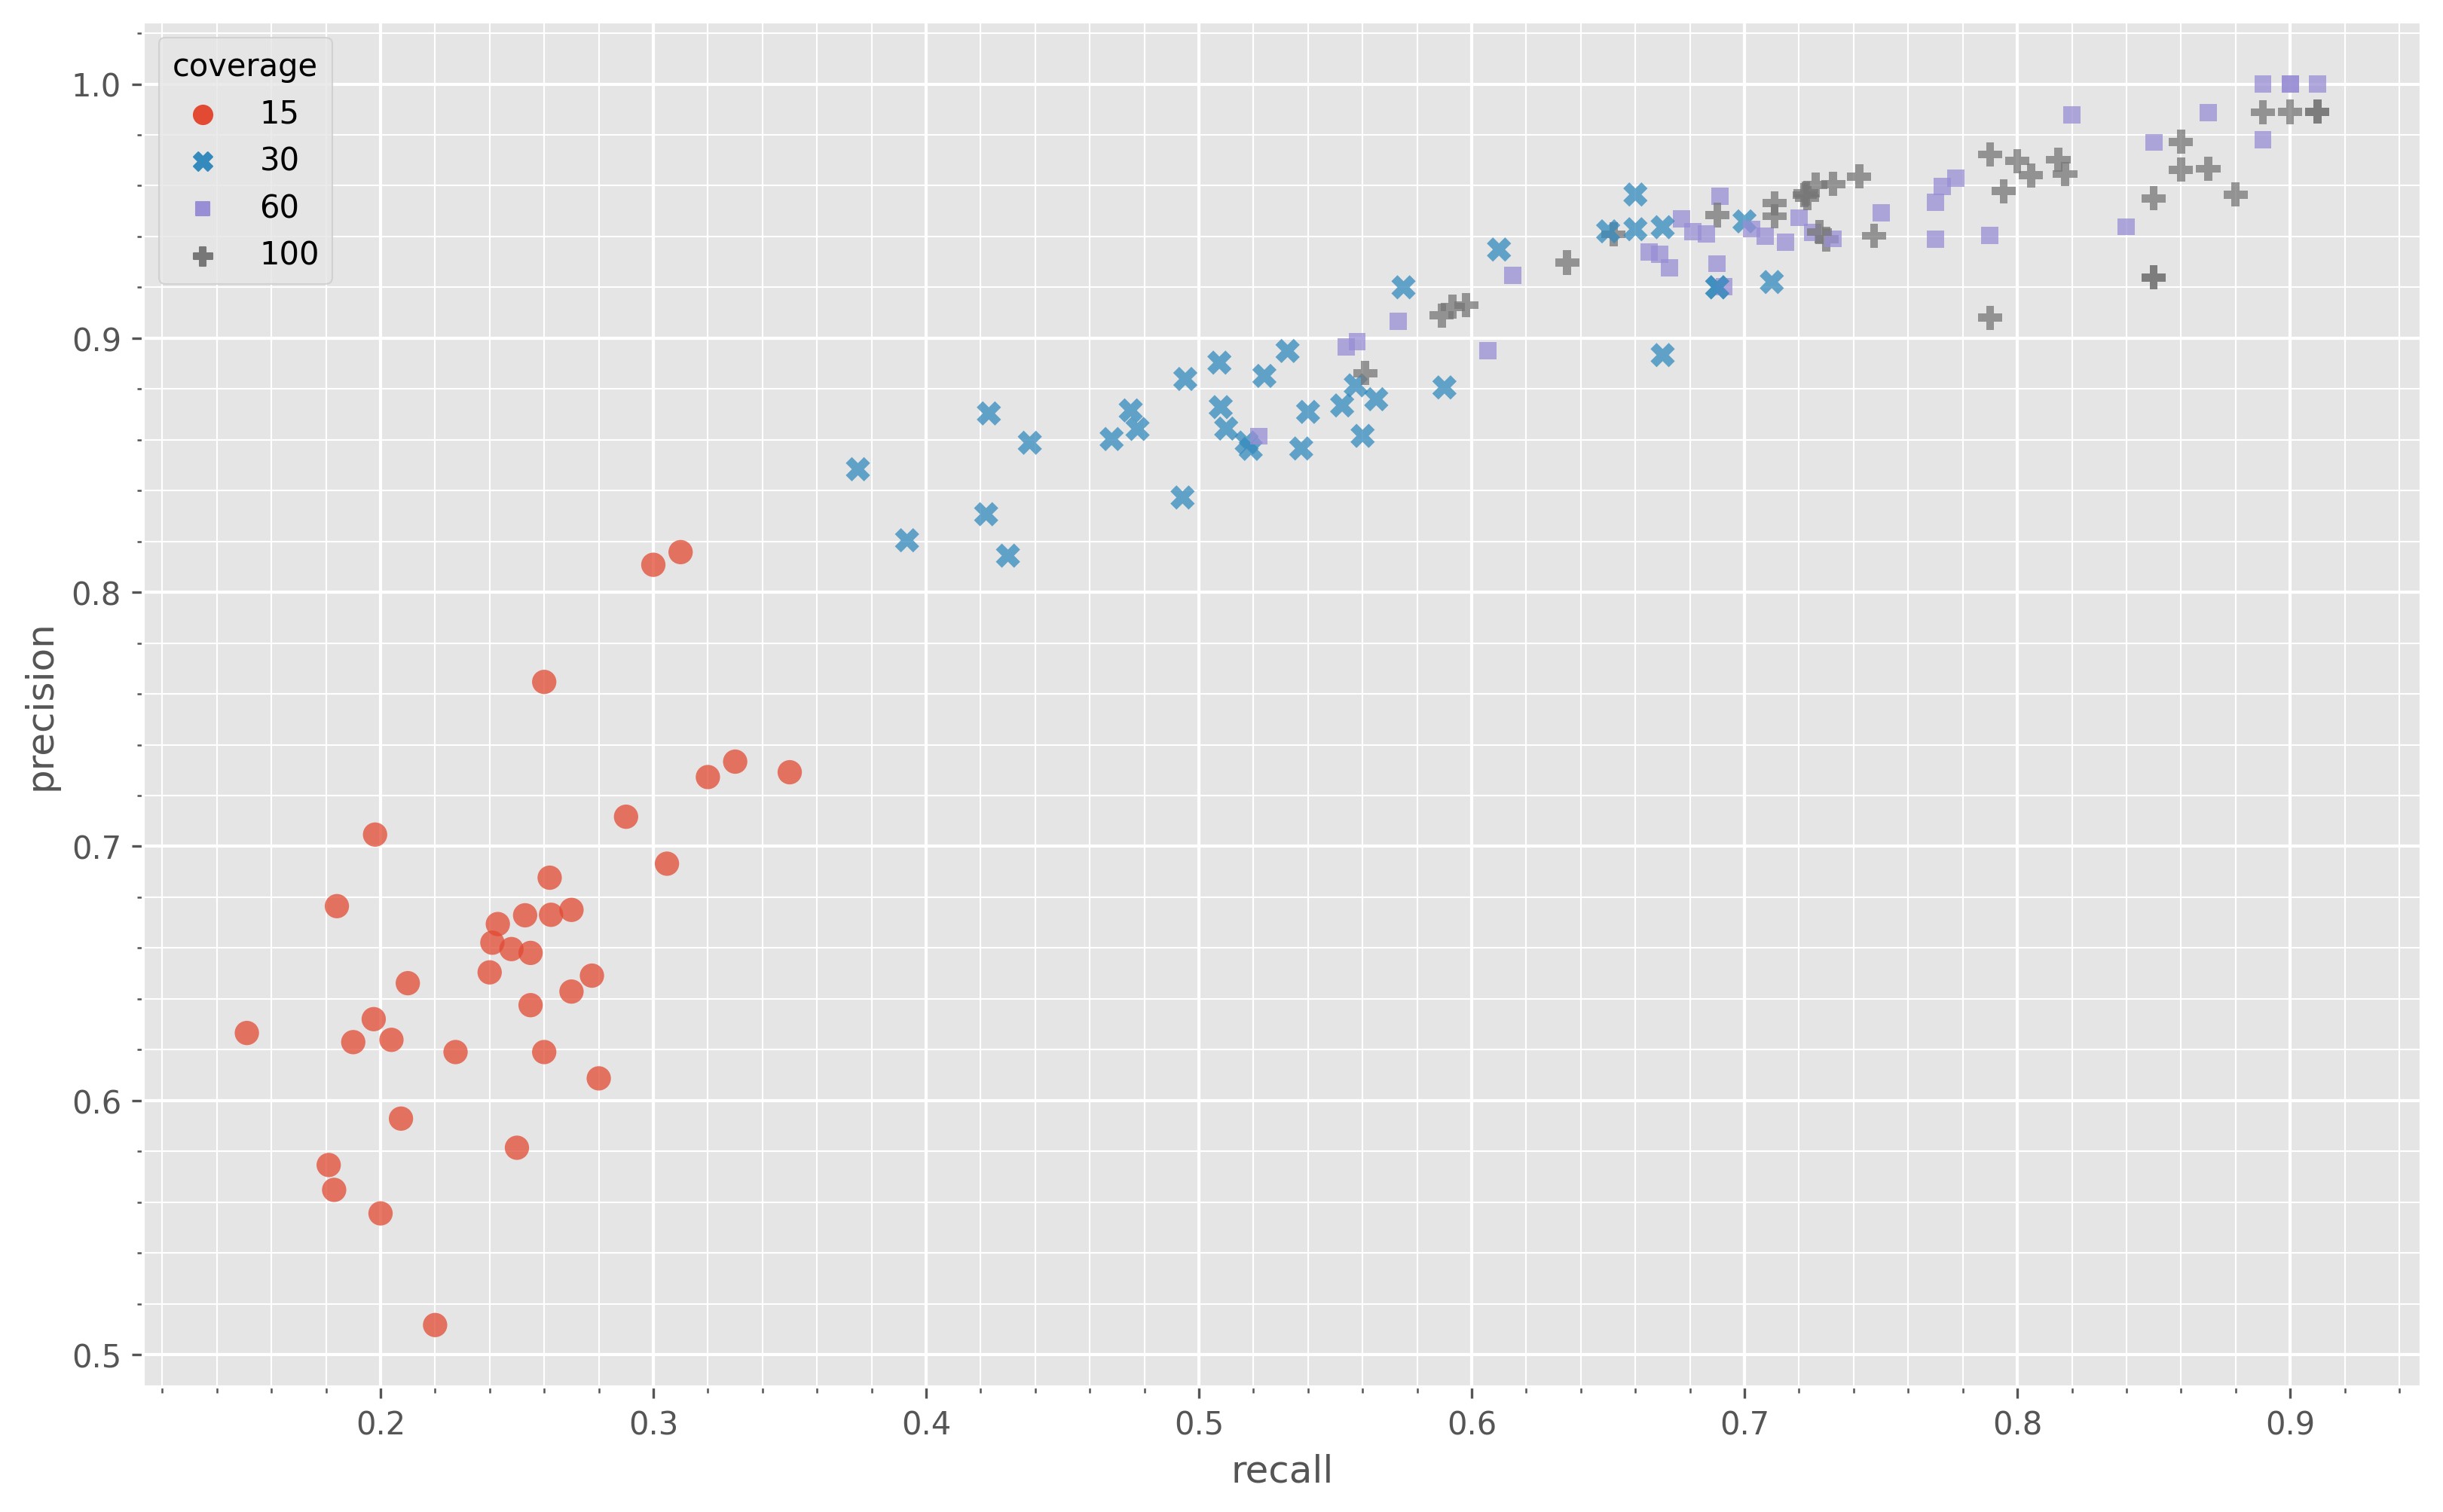
\includegraphics[width=1\linewidth]{Chapter1/Figs/denovo_precrec_covg.png}
     \end{subfigure}
     \begin{subfigure}[b]{0.475\textwidth}
         \centering
          \caption[position=above]{Number of SNPs simulated}
         \label{fig:denovo-sims-num-snps}
        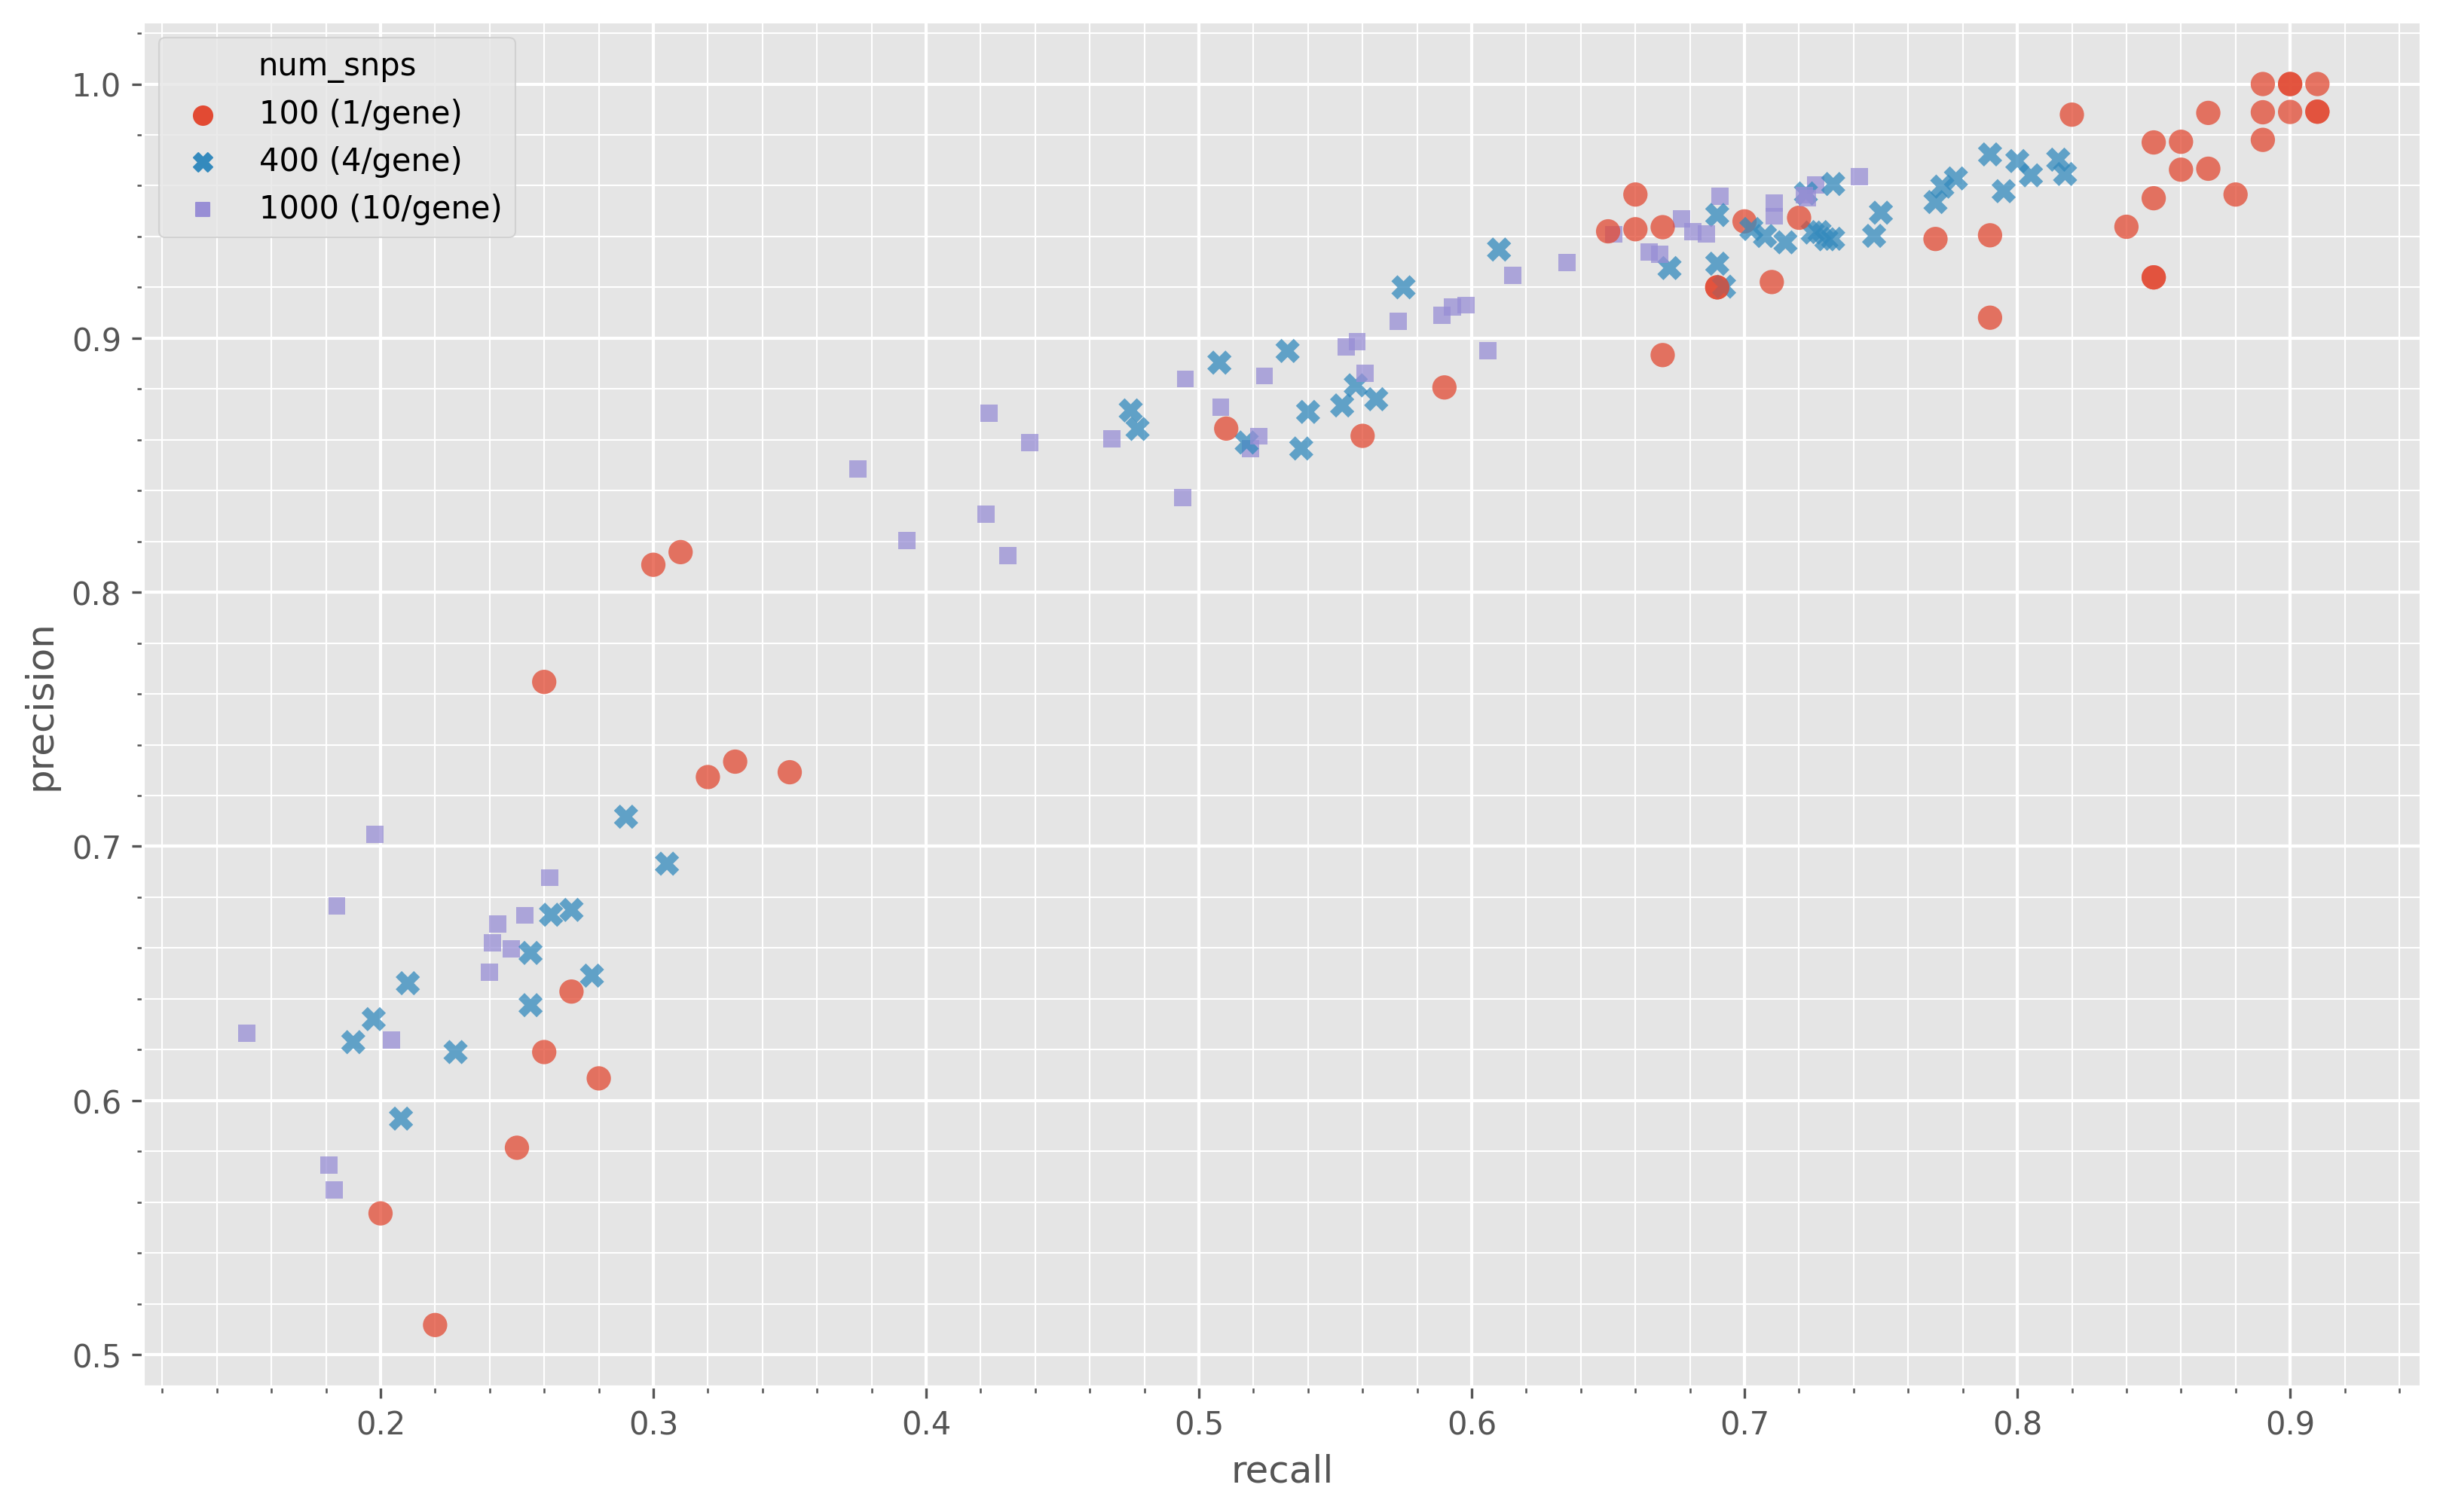
\includegraphics[width=1\linewidth]{Chapter1/Figs/denovo_precrec_num_snps.png}
     \end{subfigure}
     \begin{subfigure}[b]{0.475\textwidth}
         \centering
        \caption[position=above]{\denovo{} discovery \kmer{} size}
        \label{fig:denovo-sims-kmer-size}
        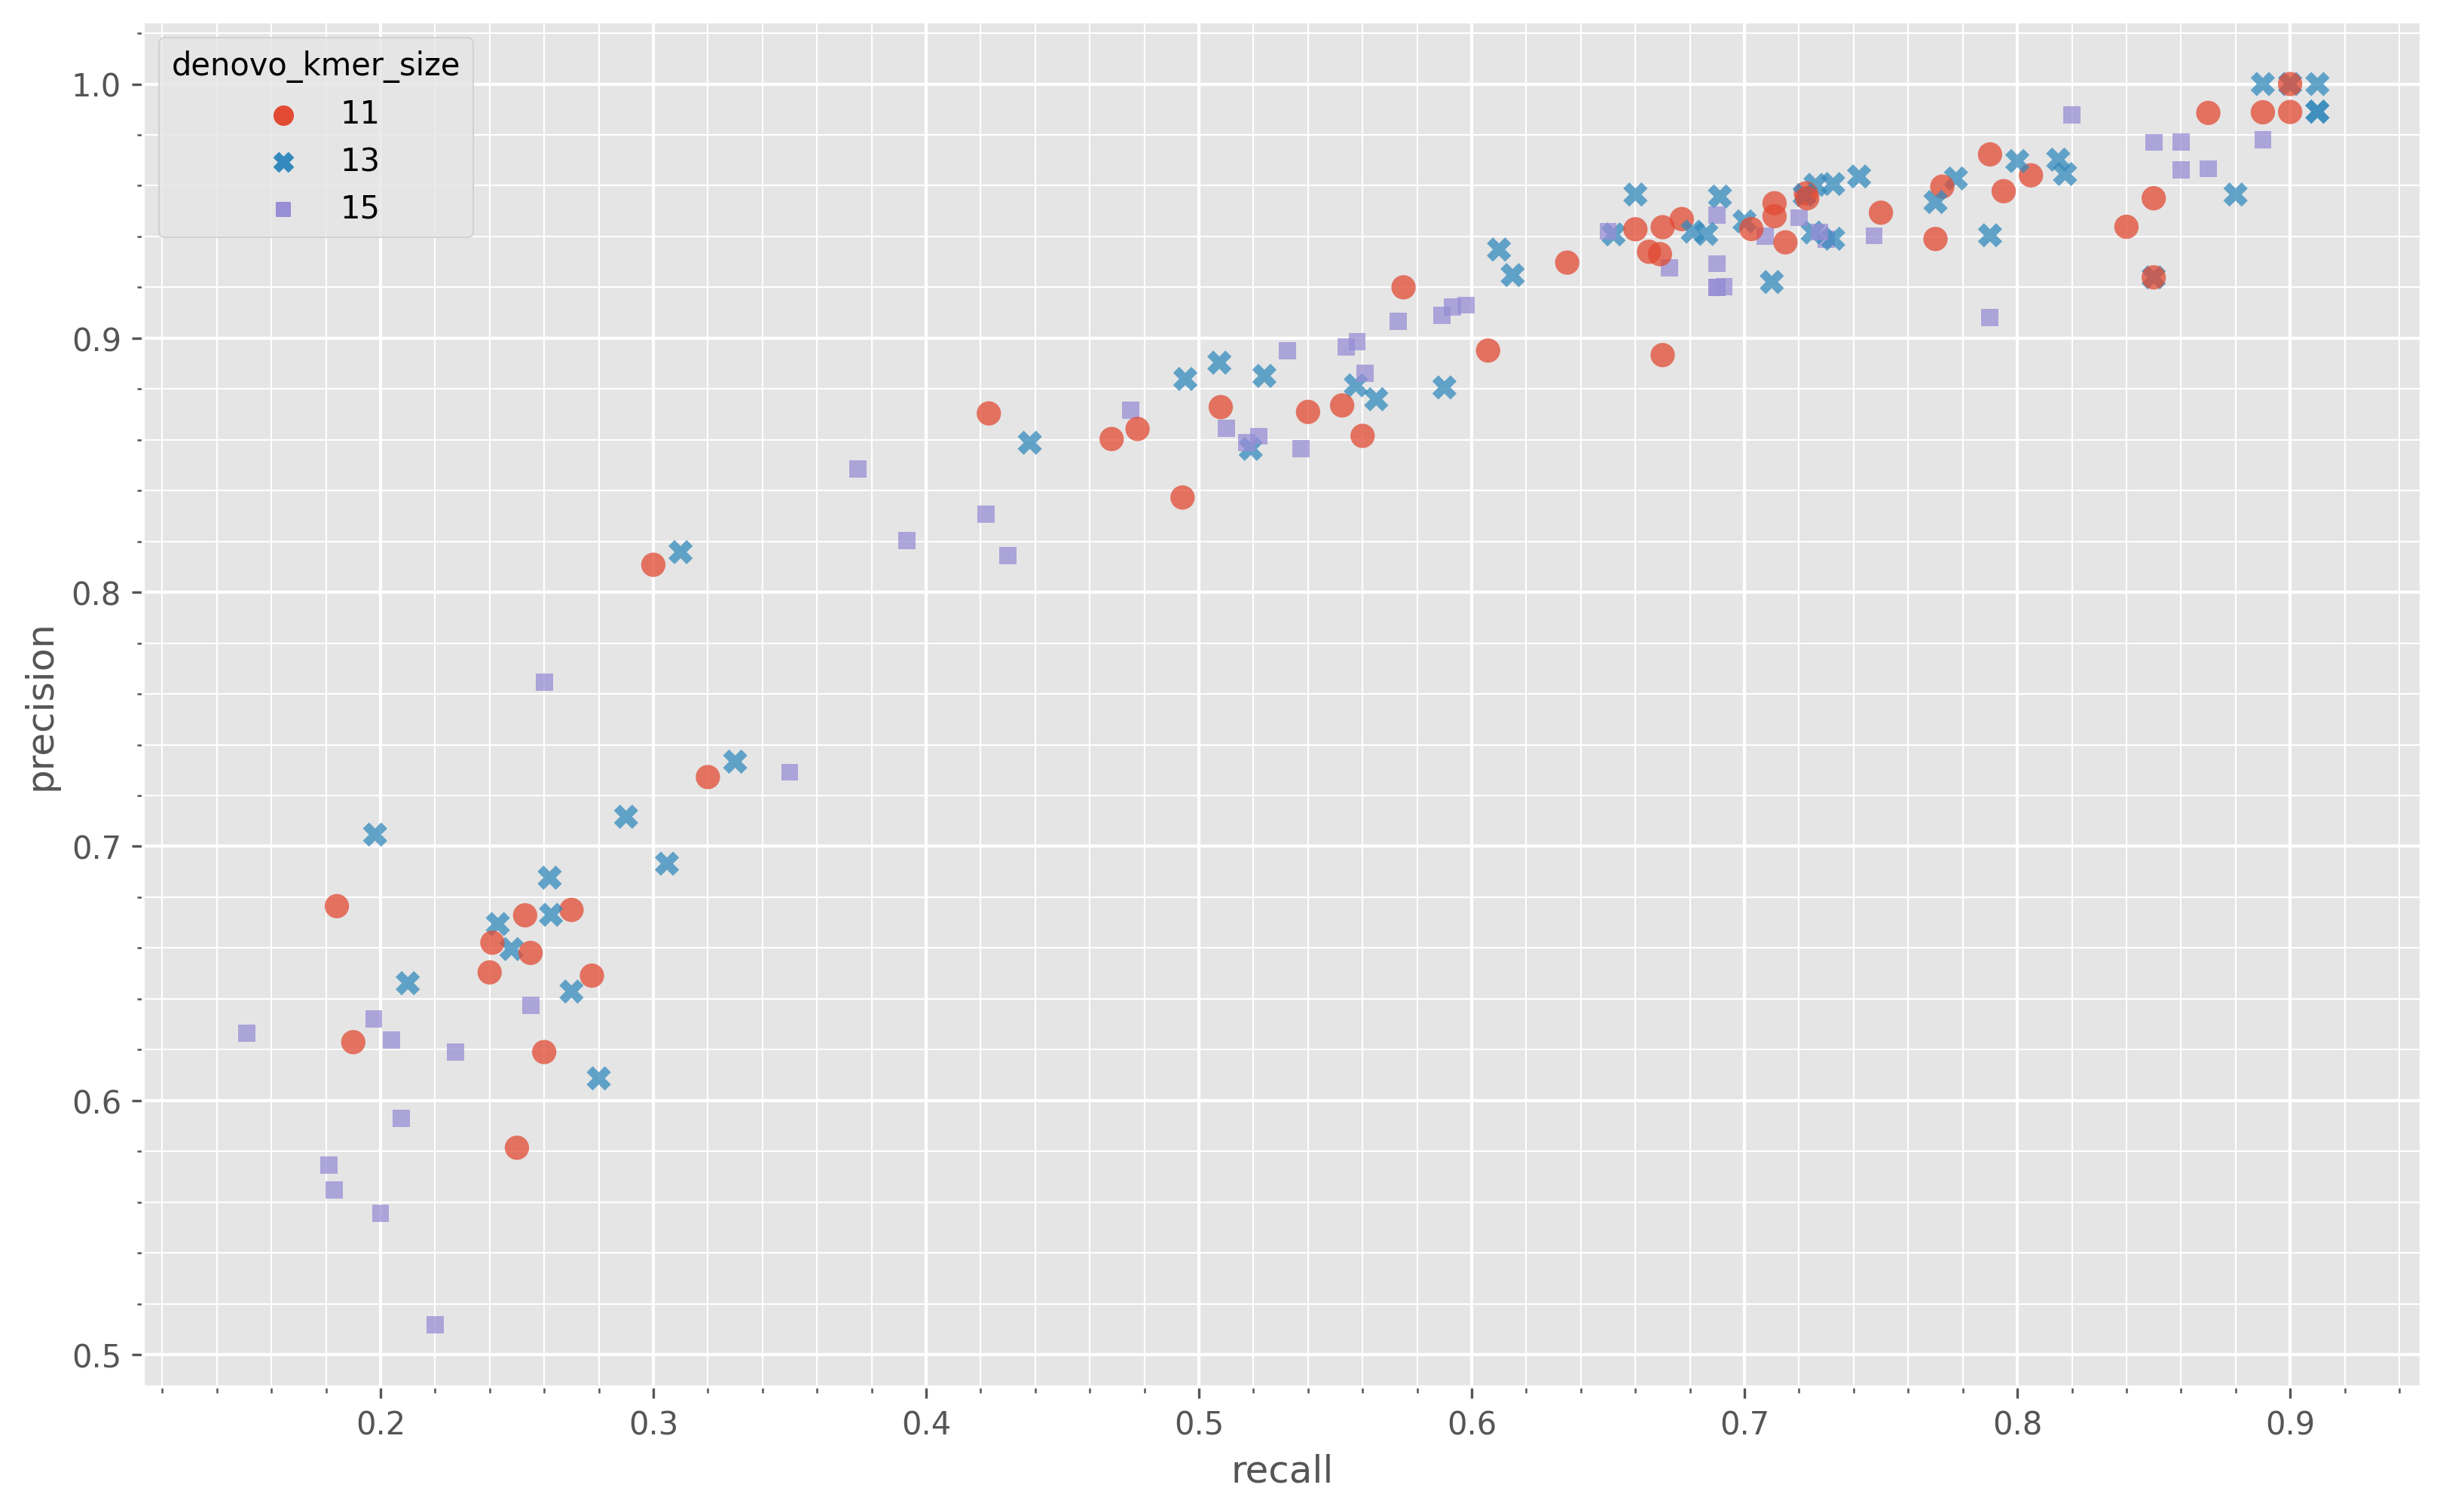
\includegraphics[width=1\linewidth]{Chapter1/Figs/denovo_precrec_kmer.png}
     \end{subfigure}
     \begin{subfigure}[b]{0.475\textwidth}
         \centering
         \caption[position=above]{\prg{} maximum nesting level}
         \label{fig:denovo-sims-nesting}
        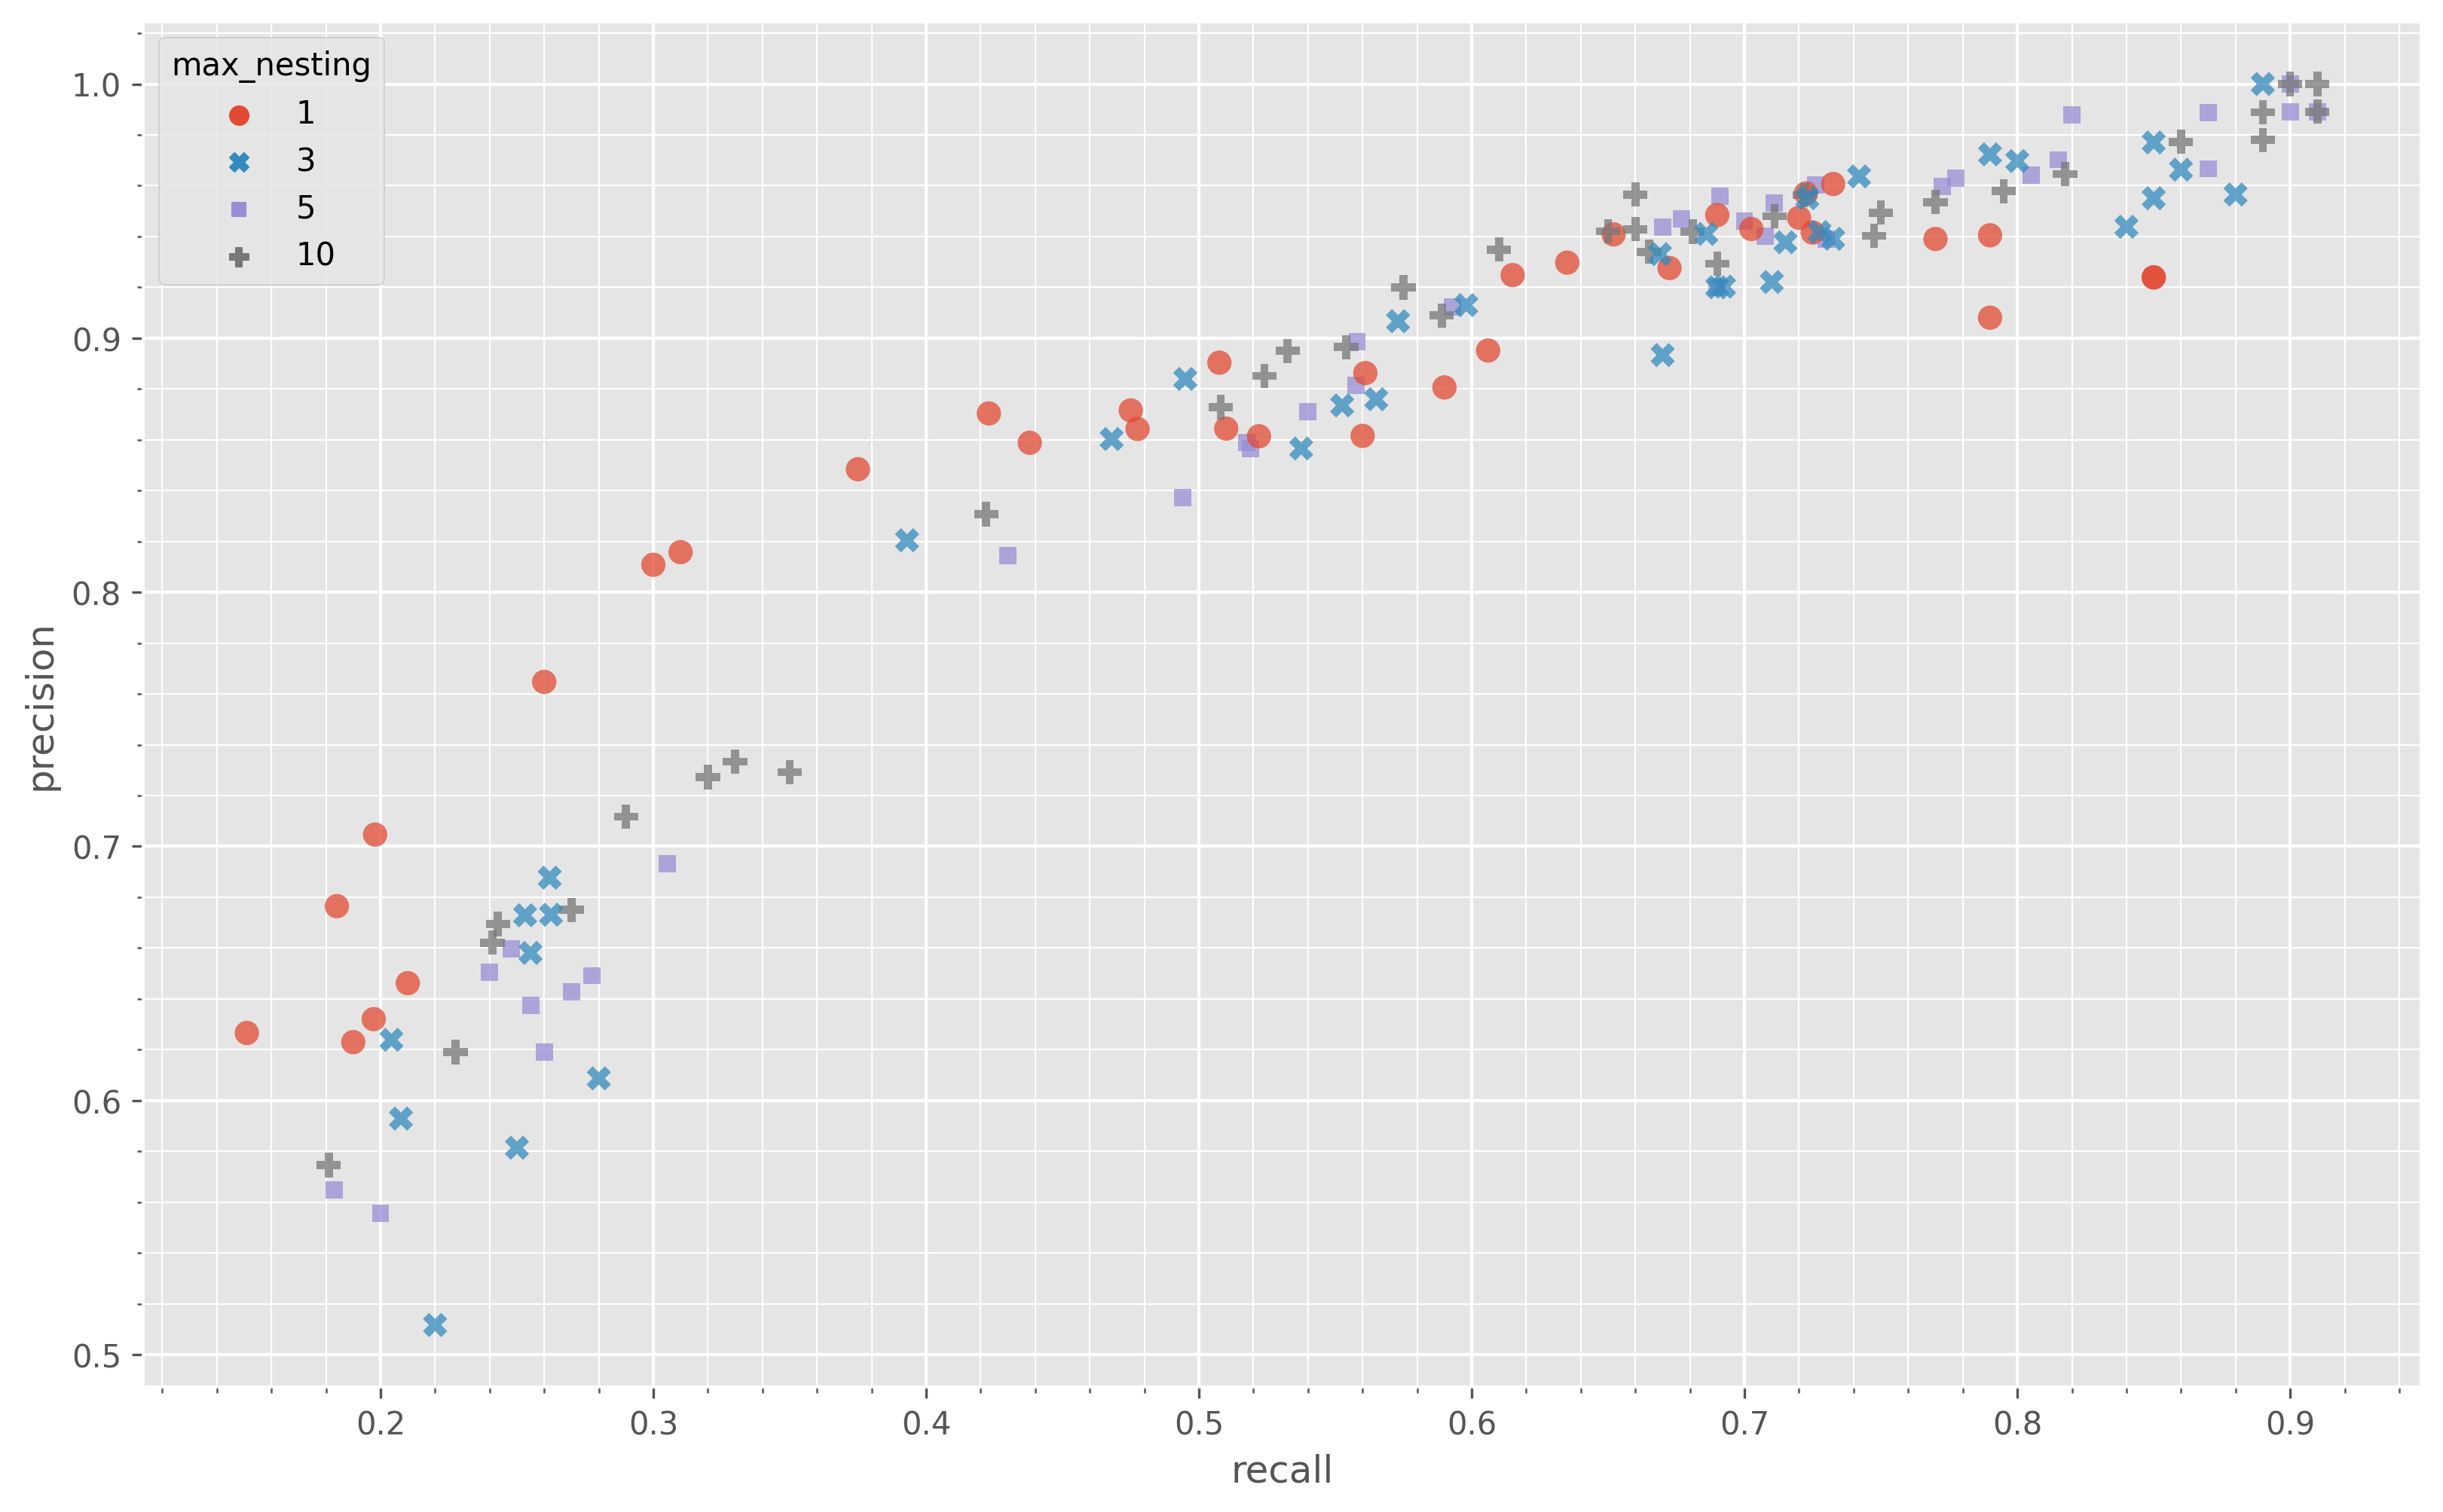
\includegraphics[width=1\linewidth]{Chapter1/Figs/denovo_precrec_nesting.png}
     \end{subfigure}
    \caption{Recall (x-axis) and precision (y-axis) of \denovo{} variants discovered by \pandora{} on a simulated dataset. Subplots style the points by the parameter indicated in the subtitle. Each point indicates a single run of \pandora{} with a unique combination of all parameters.}
        \label{fig:denovo-sims}
\end{figure}

While not an issue for the best-performing example we have just been examining, missing loci were another common source of FNs. If \pandora{} decides a locus is not present after quasi-mapping (\autoref{sec:pandora-intro}), then it is impossible for \denovo{} to discover any variants in it. We note that the vast majority of missing loci have a length of less than 250 base pairs (\autoref{app:denovo-missing-lengths}).

When looking across all 144 combinations of parameters, we found that, on average, 7.8\% of the true variants are near the ends of loci and 2.8\% are in absent loci (see \autoref{fig:denovo-errors}). 

\begin{figure}
    \centering
    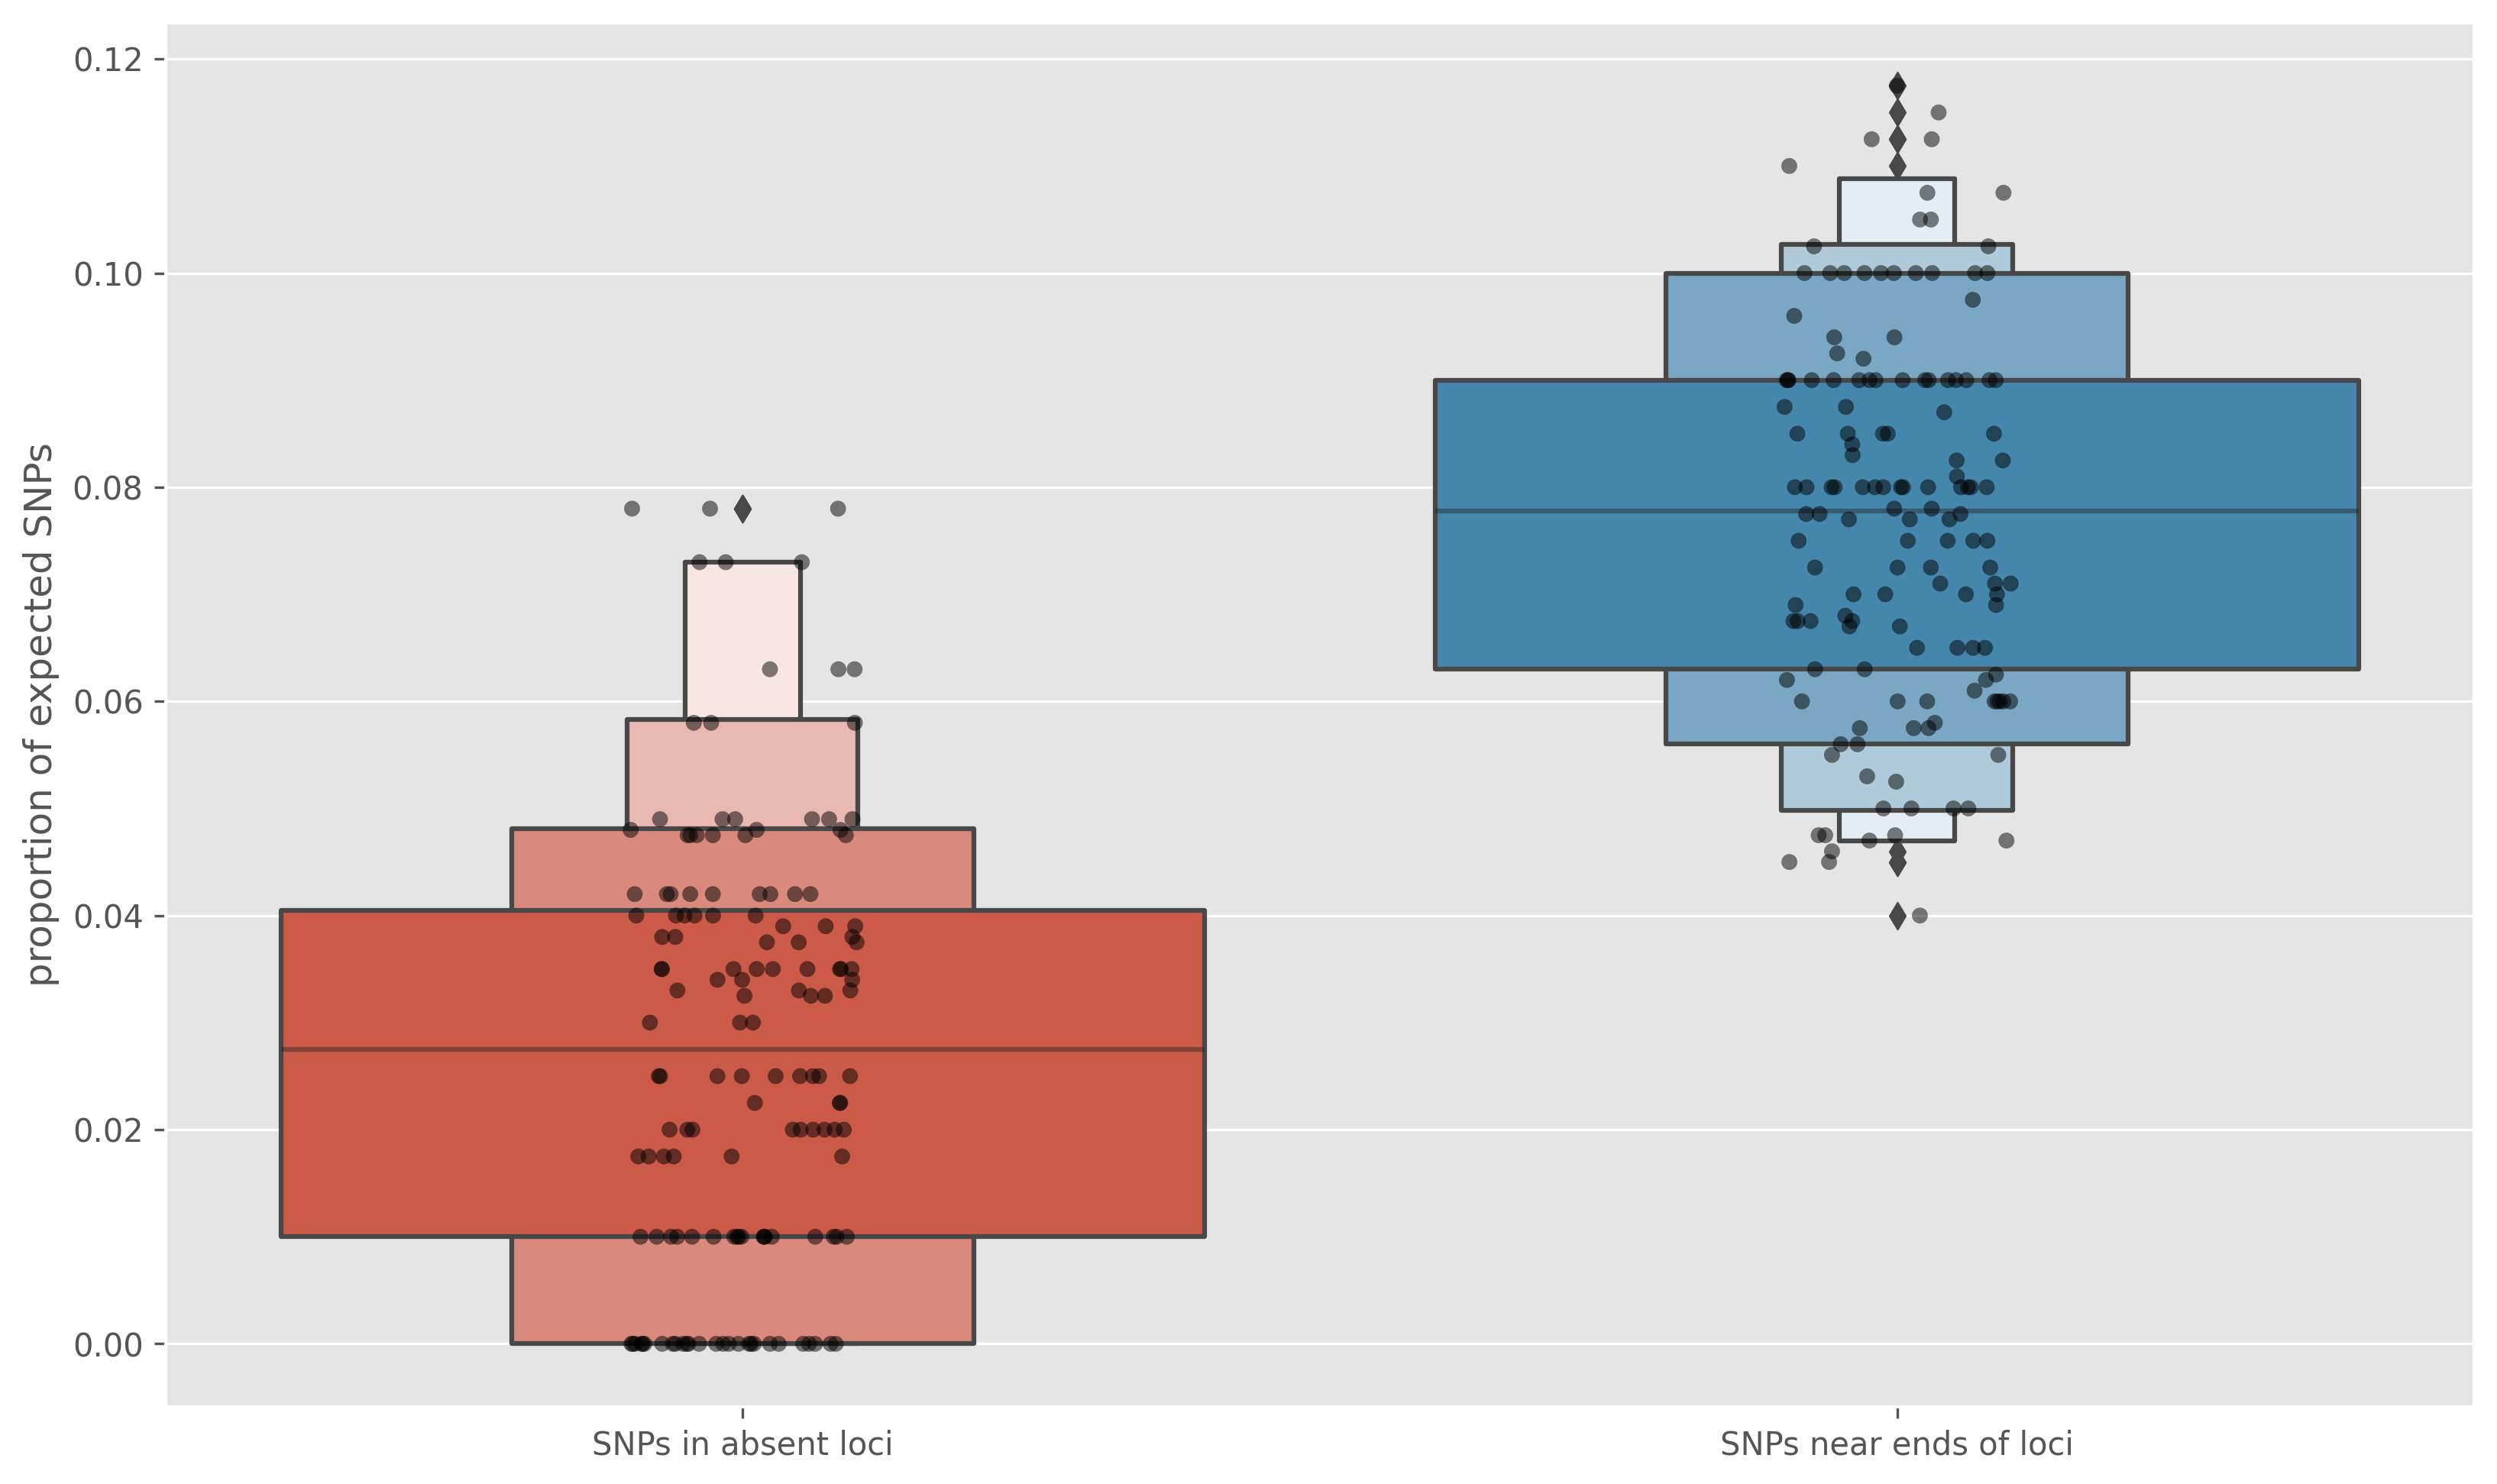
\includegraphics[width=0.9\textwidth]{Chapter1/Figs/denovo_errors.png}
    \caption{The proportion of simulated SNPs that are not detectable by \denovo{} variant discovery. The red box represents SNPs that occur in loci designated as absent by \pandora{}. The blue box depicts the SNPs that occur within $2k-1$ positions of the start or end of a locus. Each point indicates a single run of \pandora{} with a unique combination of parameters.}
    \label{fig:denovo-errors}
\end{figure}

\noindent
The parameters that we can directly control with respect to \denovo{} discovery within \pandora{} are the \prg{} maximum nesting level and the \denovo{} \kmer{} size. \autoref{fig:denovo-sims} shows no clear optimum for either of these options. However, when taking the median precision and recall values across all data points (\autoref{tab:denovo-summary}), a maximum nesting level of 5 and \denovo{} \kmer{} size of 13 seem the best choice.

\begin{table}
\centering
\begin{tabular}{@{}lll@{}}
\toprule
          & Max. nesting & \denovo{} \kmer{} size \\ \midrule
Precision & 0.934 (10)   & 0.937 (13)                                               \\
Recall    & 0.674 (5)    & 0.671 (13)                                               \\ \bottomrule
\end{tabular}
\caption{The median precision and recall for all parameter combinations, grouping by the maximum \prg{} nesting level or the \denovo{} \kmer{} size used for variant discovery in \pandora{}. The values in parentheses indicate the parameter value that leads to the specified precision or recall.}
\label{tab:denovo-summary}
\end{table}

For the final analysis of the simulation data, we look at how the precision and recall change with an increasing genotype confidence threshold. We select the data point with the optimal maximum nesting level (5) and \denovo{} \kmer{} size (13), along with 4 SNPs per gene, as this is within the range expected for an \ecoli{} genome. Next, starting at 0 and increasing by 10 until 700, we filter out any variant with a genotype confidence score below the current threshold. The purpose of this analysis is to illustrate what the cost on recall is for requiring more confident variant calls at different read depths.

\autoref{fig:denovo-sims-roc} shows the same relationship we saw earlier: coverage has a significant impact on precision and recall. Most importantly, though, it shows that the inclusion of \denovo{} discovery is vital for finding novel variants. Precision and recall for \pandora{} \emph{without} variant discovery are not shown in \autoref{fig:denovo-sims-roc}, as the best recall achievable for this set of parameters was only 1.0\% (indicating that 4 SNPs were incidentally in the \panrg{}). This is compared to a maximum of 81.5\% when using \denovo{} discovery. Focusing on the 100x coverage data point with \denovo{} discovery, the best recall (81.5\%) leads to a precision of 97.0\%, but the cost of increasing precision to 99\% is decreasing recall to 25\%. 

\begin{figure}
    \centering
    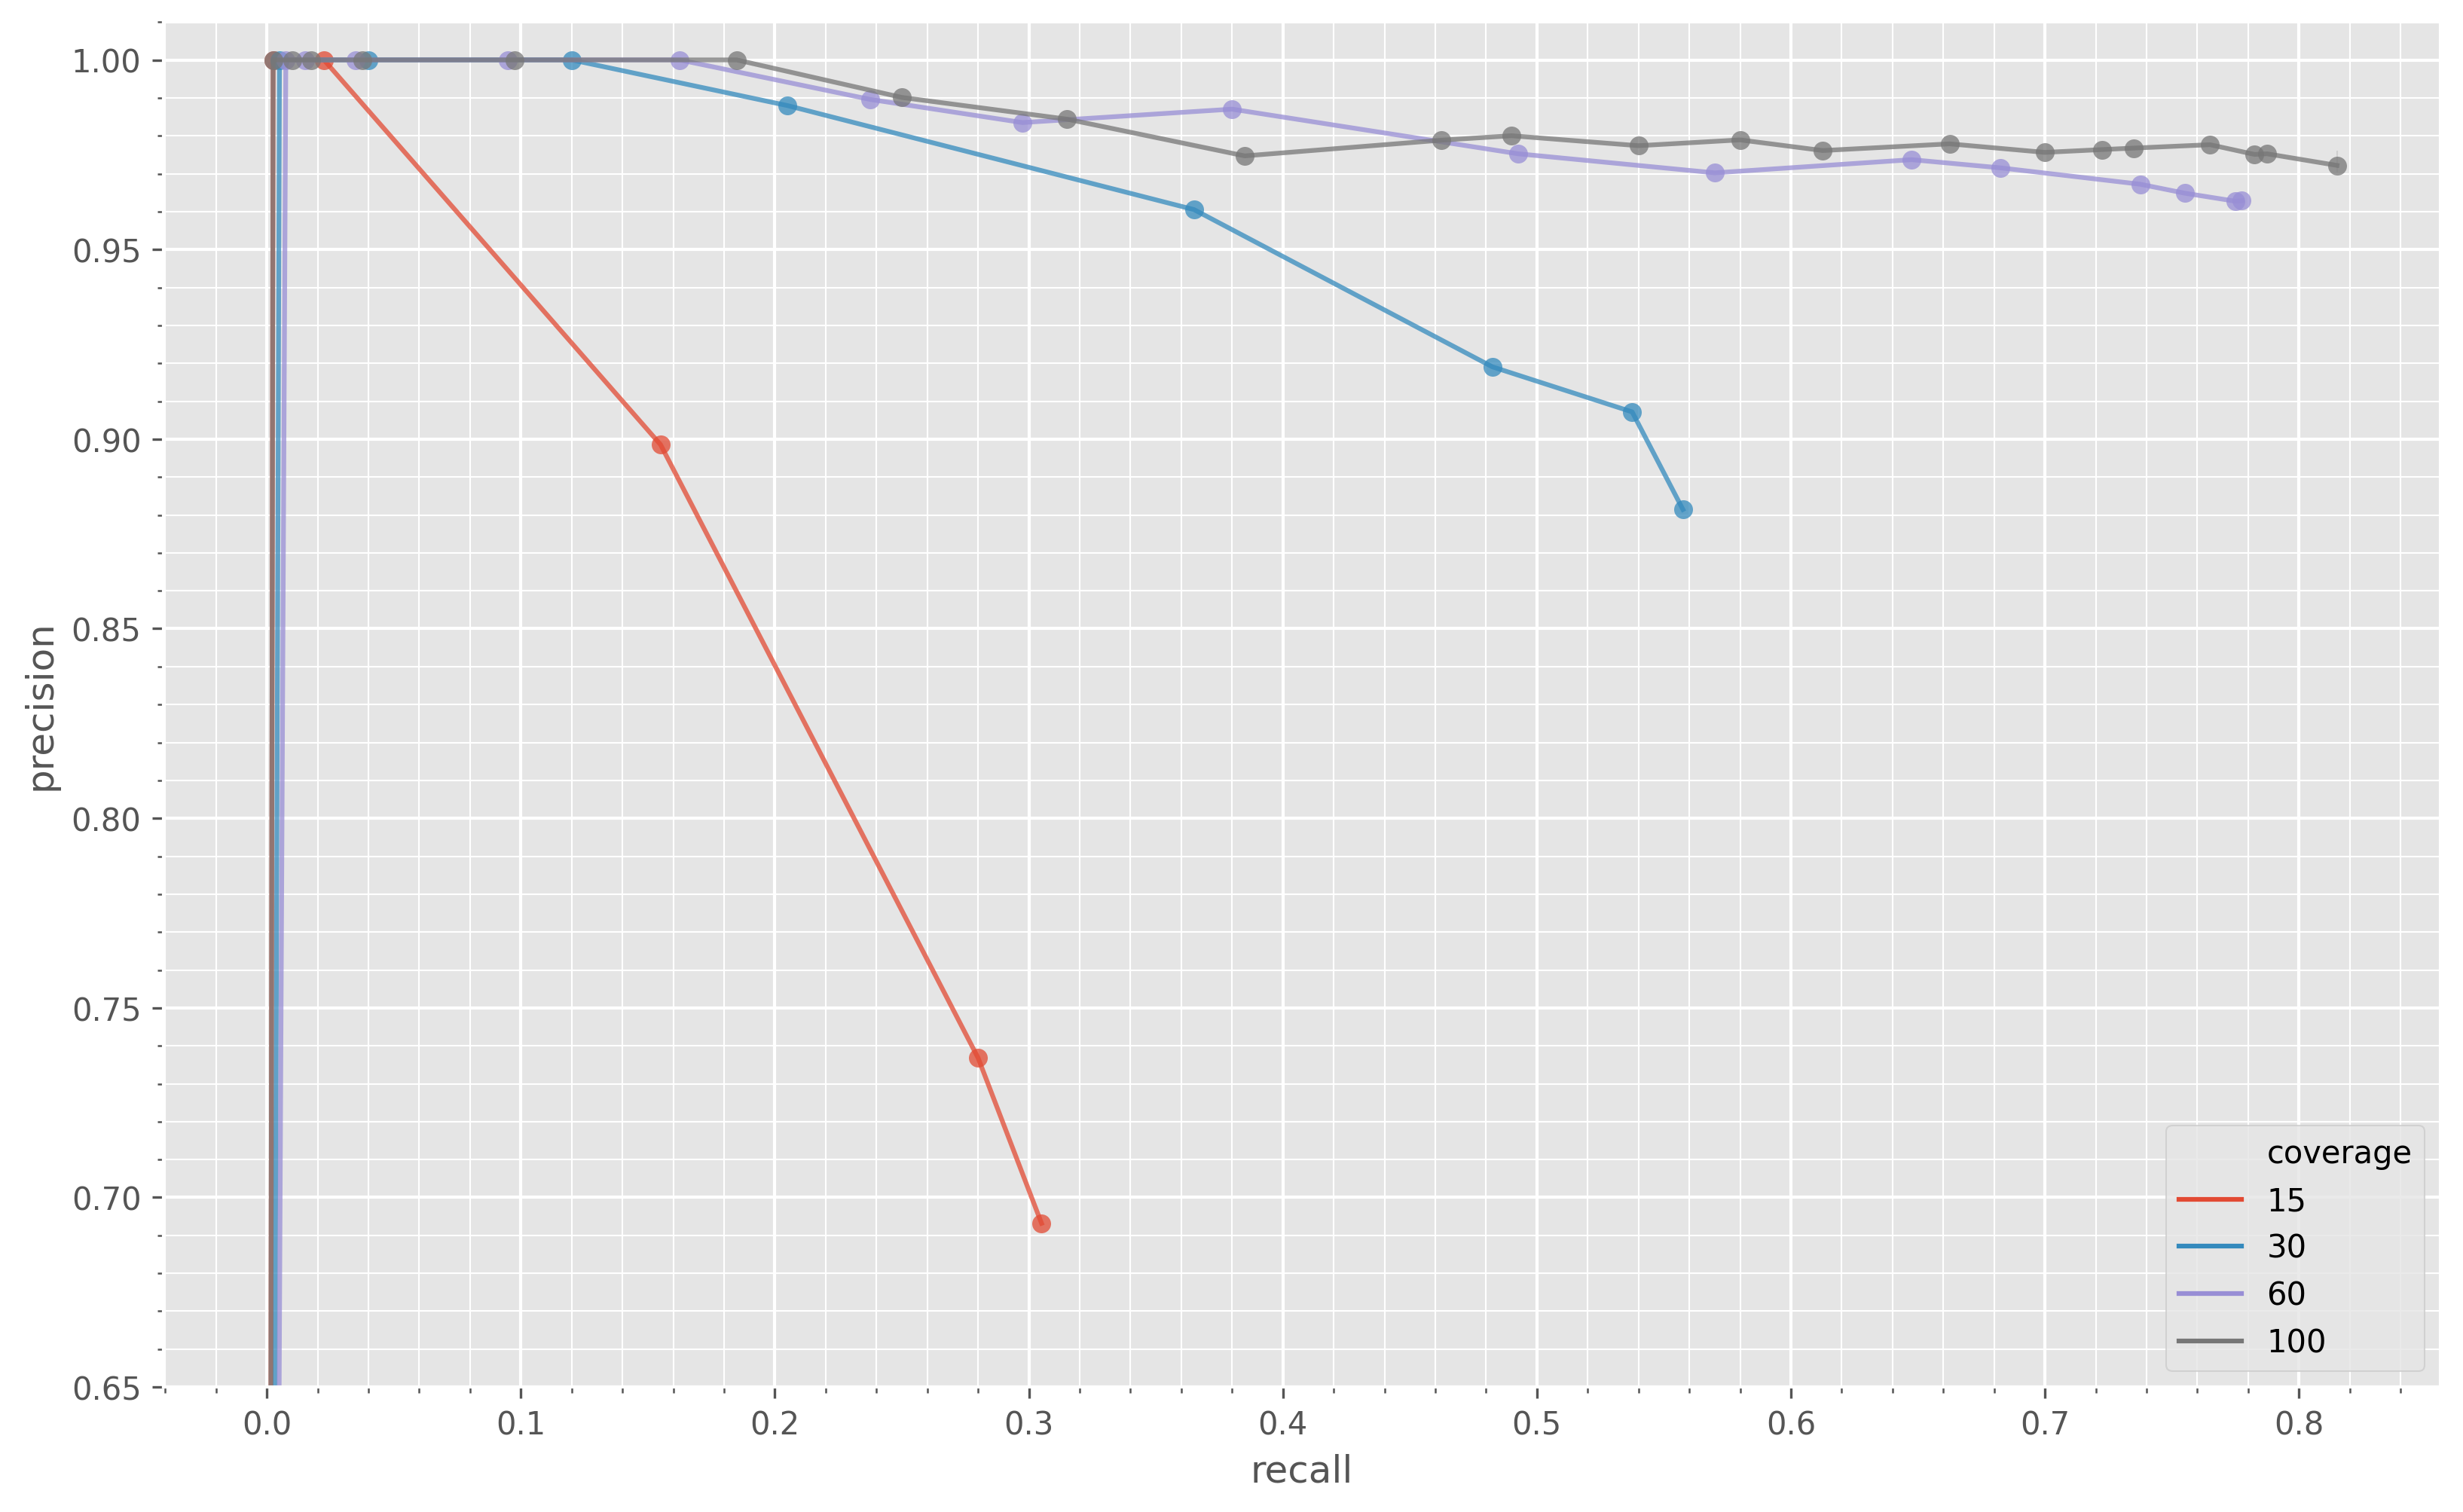
\includegraphics[width=0.9\textwidth]{Chapter1/Figs/denovo-sims-roc.png}
    \caption{Precision-recall curve for increasing genotype confidence score thresholds. The curves are coloured by read depth (coverage). Each marker/point is a different genotype confidence threshold, starting with 0 as the right-most value and increasing as the line moves towards the (top) left. Note, the y-axis has been cut to provide more clarity of precision.}
    \label{fig:denovo-sims-roc}
\end{figure}

\subsection{Summary}

In summary, we have shown that the addition of the \denovo{} variant discovery method outlined in \autoref{sec:denovo-method} gives \pandora{} the ability to find many variants not present in its \panrg{}. Using simulated data, we find a \kmer{} size of 13 gives slightly better recall than 11 or 15, but that the sample read depth has the most considerable impact on our ability to discover novel variants.

We have also shown that, on average, approximately 10.5\% of (simulated) SNPs are not detectable based on their membership in either loci \pandora{} does not detect, or lying within $2k-1$ positions of the start or end of a locus.

% ==================================================================
\section{Validation with empirical data}
\label{sec:denovo-empirical}

Having shown, for simulated data, that the \denovo{} variant discovery method indeed alleviates a major limitation of \pandora{}, we turn our attention to evaluating its performance on empirical data. However, rather than the single-sample (\pandora{} \vrb{map}) approach we used for genotyping in \autoref{sec:denovo-sims}, we evaluate \pandora{}'s multi-sample comparison protocol - \compare{}.

The inference of variation within a collection of samples is one of the unique aspects of \pandora{}. As detailed in \autoref{sec:pandora-compare}, the \vrb{compare} routine of \pandora{} genotypes multiple samples against a \panrg{} simultaneously, with the aim of representing variation between the samples in the most succinct manner possible (see \autoref{fig:var-representation}). It does this by selecting a single maximum likelihood path that best approximates the samples under investigation - akin to an "average" path of the samples.

Evaluating the variant calls from such a graph-based method is by no means trivial. In this section, we aim to compare the variant calls made by \pandora{} against those made by single-reference (linear) methods for both Illumina and \ont{} data.

In keeping with the focus of this chapter, we will also assess the utility of \denovo{} variant discovery within \pandora{}. While we have shown its benefit on simulated data, the \panrg{} used did not contain many of the simulated SNPs. However, we expect many of the SNPs in real data also to be present in a \panrg{} built from a pan-genome of diverse samples. 

\textit{Note: all work in this section (\autoref{sec:denovo-empirical}) is described in full in \cite{pandora}. See \autoref{sec:denovo-acknowledge} for a detailed description of what work was completed by myself.}

\subsection{Dataset}
\label{sec:denovo-empirical-data}

\subsubsection{Samples}
The empirical data we use for this evaluation is a diverse set of 20 \ecoli{} samples from four different phylogroups. Each sample has both \ont{} and Illumina sequencing data and high-quality assemblies available. The sequencing reads for each technology were subsampled to read depth 100x.

\subsubsection{References}
The \panrg{} we use as the reference for \pandora{} was constructed from a combination of \ecoli{} genes and intergenic regions. 23,054 gene MSAs from 350 RefSeq genomes were obtained from the panX database \cite{panx}, while 14,374 intergenic region MSAs from 228 ST131 genomes were collected from \cite{thorpe2018}. \prg{}s were constructed for each locus using \makeprg{} and then all were combined into a single \panrg{} file and indexed with \pandora{}.

As single-reference variant callers cannot use a \panrg{}, we selected 24 reference genomes from five major phylogroups - one phylogroup is not contained within the sample set. These references were selected to be spread across phylogroups, and where the phylogroup was present in our samples, we chose the nearest RefSeq genome according to Mash, and a phylogenetic tree \cite{pandora}. By calling variants for each sample with respect to each reference genome, we can directly view the impact of reference selection on the results of standard variant callers.

\subsection{Variant calling}

\subsubsection{Graph-based: Pandora}
To produce a multi-sample VCF file of variants for \pandora{} we follow a somewhat similar approach to \autoref{sec:denovo-sims-methods}, with some important differences. Rather than adding all \denovo{} variants for a single sample to the original \panrg{} we instead add the novel variants for \emph{all} samples to the original \panrg{}. In the end, we have an updated \panrg{} which contains all novel variants for all samples under comparison. We then perform multi-sample genotyping with this updated \panrg{} using \compare{}. This entire process is completed separately for Illumina and \ont{} data.

\subsubsection{Linear-based}
We compare the Illumina variant calls from \pandora{} against those from Samtools \cite{samtools2009} and Snippy (\url{https://github.com/tseemann/snippy}) (which is a wrapper around Freebayes \cite{Garrison2012}). The \ont{} variant callers we evaluate against are Medaka (\url{https://github.com/nanoporetech/medaka}) and Nanopolish \cite{Loman2015}. Each variant caller is run on all 20 samples with all 24 reference genomes. 

\noindent
In total, we produce 480 VCFs for each linear variant caller and 20 (one per sample) for \pandora{}.

\subsection{Evaluation}
\label{sec:denovo-empirical-eval}

A direct comparison of the VCF files produced by \pandora{} and the single-reference tools is not possible due to coordinate incompatibilities. As such, we use a probe-based method, akin to that in \autoref{sec:denovo-sims-eval} for assessing the variant calls. 

The first step in this evaluation is the generation of a pan-genome SNP truth set. \autoref{app:pangenome-snp-truth} details the construction of this truth set, resulting in 618,305 SNPs we expect to find amongst the 20 samples.

There are two measures of recall in a pan-genome (see \autoref{app:pangenome-snp-truth}), but of interest to this section is the average allelic recall (AvgAR). Briefly, AvgAR is the average recall of all pan-genome variants. For example, we have three genomes with two pan-genome variants $P_1$ and $P_2$ between them. $P_1$ has the alleles A, A, and T across the three genomes, and $P_2$ has alleles C, T, and T. If we find the $P_1$ alleles A (for only one sample) and T, we have a $P_1$ recall of 0.66 (2/3), and if we only find the $P_2$ allele C, we have a $P_2$ recall of 0.33 (1/3). Therefore, in this example, we have an AvgAR of $\frac{0.66+0.33}{2}=0.5$.

To calculate AvgAR (recall) for tool-reference pairs, we perform the following: i) apply the variant calls for each sample to the reference sequence the calls were made with respect to (giving 20 mutated sequences); ii) we map all truth set probes to these mutated reference sequences with \vrb{bwa mem}; iii) we classify a mapping as TP if the alleles within the aligned sequences match. Then, for each pan-genome variant, we count the proportion of its alleles with a TP mapping and calculate AvgAR accordingly. In the end, we have an AvgAR value for each variant caller and reference sequence combination - i.e., 24 AvgAR values for each caller.

We determine precision in a somewhat similar manner. First, we create probes for each variant in a given VCF, with 150bp of flanking sequence taken from the VCF reference sequence. Second, we map each probe to the sample's assembly sequence. Next, we filter out poor quality mappings or mappings to low-quality regions of the assembly. Finally, each mapping's precision is classified as a continuous score - rather than a binary true or false positive - by dividing the number of matching bases (ignoring the flanking sequences) by the alignment length. Thus, for example, if the called allele is ATG and maps to a sequence ATTG, the precision score is 0.75. Ultimately, we calculate precision as the sum of precision scores, divided by the number of evaluated calls.

\subsection{Effect of different \ont{} basecalling models}
\label{sec:denovo-methylation}

Previous work from Wick \etal{} has shown that for Enterobacteriaceae, the majority of \ont{} sequencing errors are related to Dcm methylation sites \cite{wick2019}. In version 3.2.1 of \guppy{} (the ONT-provided basecalling software) a new \emph{methylation-aware} model was made available. However, this new model is considerably slower to basecall reads than the default model. As \ecoli{} is a member of this family, we set out to test a subset of 4 samples from our dataset to see whether a methylation-aware model indeed has a noticeable impact on the precision and recall from \pandora{} - with and without \denovo{} variant discovery.

We basecalled the raw data for four samples from our dataset with both the default and methylation-aware models from \guppy{} version 3.4.5. Precision and recall (AvgAR) are calculated as per \autoref{sec:denovo-empirical-eval} and presented in \autoref{fig:denovo-methylation}. 

The precision-recall curves represent increasing genotype confidence filtering; the top-right of each curve is no filtering, and as the genotype confidence requirement is gradually increased, we reduce the error rate (increase precision) at the loss of recall. 

Two crucial observations from \autoref{fig:denovo-methylation} are that the use of a methylation-aware model increases both precision \emph{and} recall, and the use of \denovo{} discovery increases recall at the cost of precision. 

\autoref{tab:denovo-methylation} shows the precision and recall values for the unfiltered results (i.e., the top-right of each curve in \autoref{fig:denovo-methylation}). From this, we see that without \denovo{} variant discovery, using a methylation-aware model would allow us to recover 894.7 variants in 1000 - 3.3 more than with the default model; likewise, we would expect to make 0.5 errors per 1000 variants. Using \denovo{} variant discovery, the methylation-aware model allows us to discover 906.3 variants in 1000 - 4.8 more than the default model and 11.6 more than methylation-aware without \denovo{} discovery. In terms of errors, using a methylation-aware model leads to 3.7 less errors per 1000 variants with novel variant discovery enabled; however, it makes 0.41 more errors per 1000 variants than without novel variant discovery. 

\begin{figure}
    \centering
    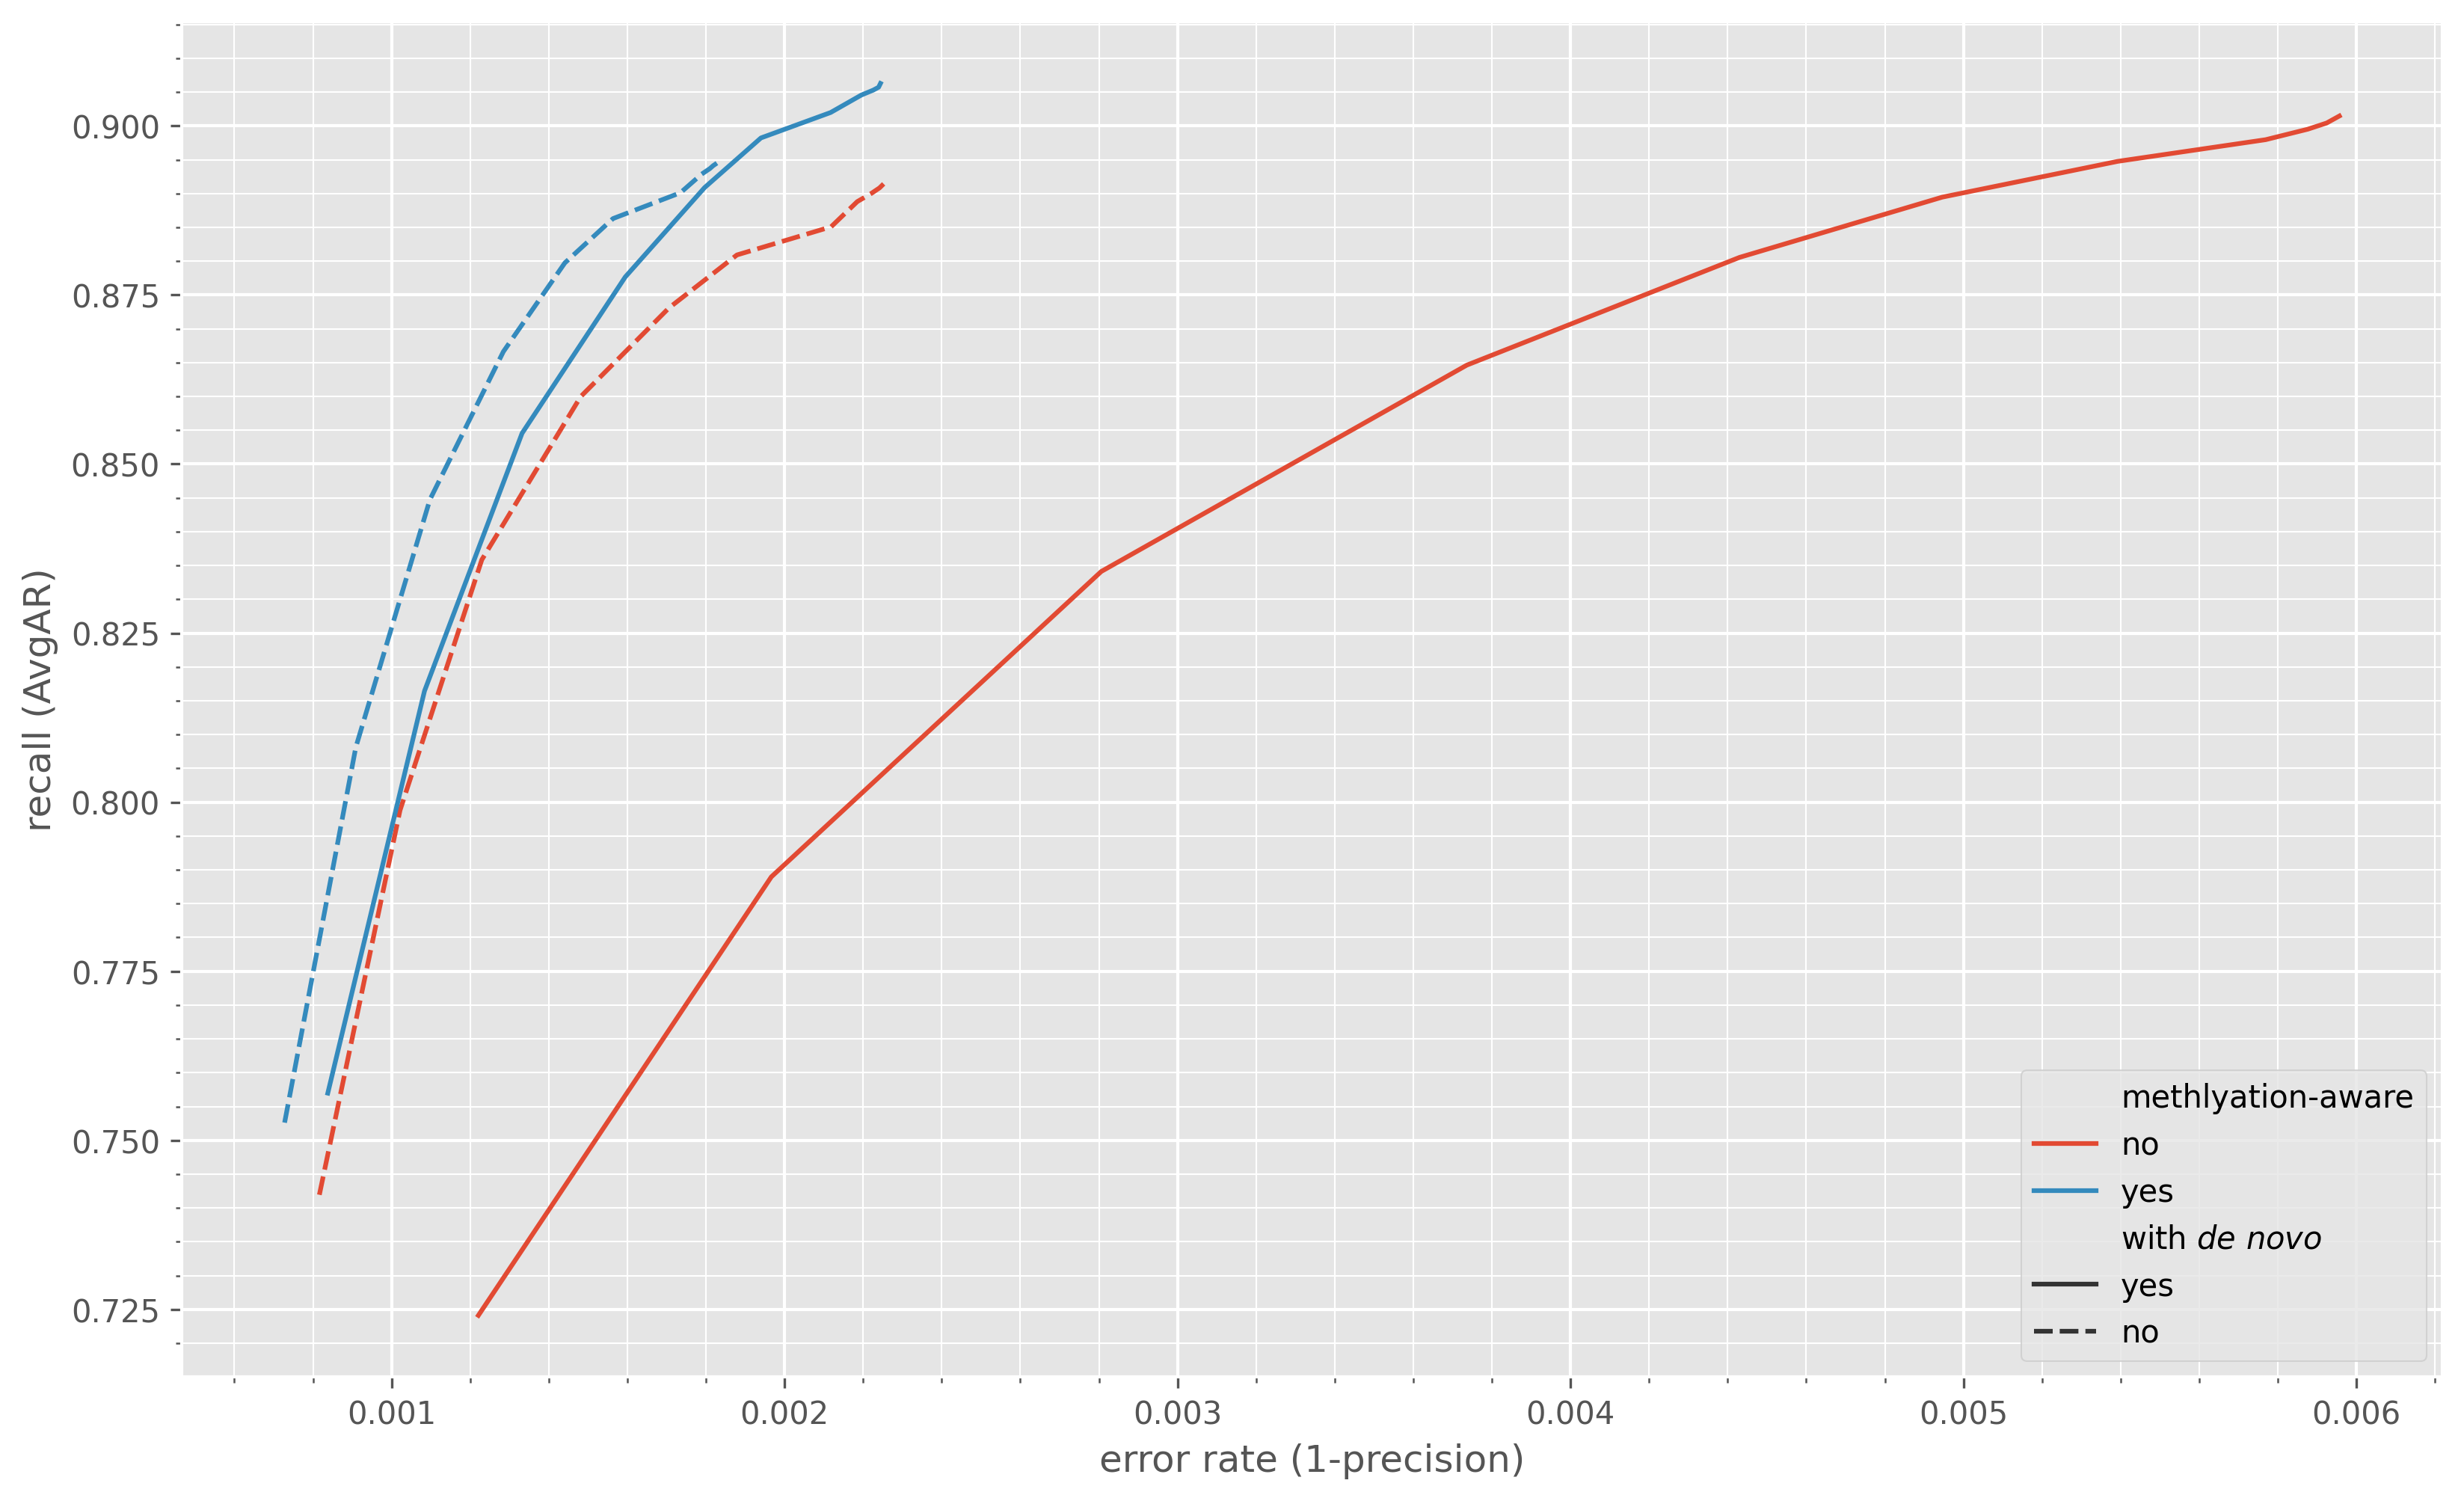
\includegraphics[width=0.9\textwidth]{Chapter1/Figs/pandora_basecaller_roc.png}
    \caption{Effect of \ont{} methylation-aware basecalling on \pandora{} \denovo{} variant discovery. The lines show the average allelic recall (AvgAR; y-axis) and error rate ($1-$precision; x-axis) of \pandora{} with increasing genotype confidence score thresholds with (solid line) and without (dashed line) \denovo{} variant discovery. The red line shows data basecalled with the default \guppy{} model and blue being basecalled with a methylation-aware model.}
    \label{fig:denovo-methylation}
    \source{Adapted from \cite{pandora} under the terms of the \href{https://creativecommons.org/licenses/}{Creative Commons CC BY license}. The colour scheme has been altered, along with the wording of some labels. However, none of these changes in any way alters the underlying data or interpretation of that data.}
\end{figure}

\begin{table}
\centering
\begin{tabular}{@{}llrr@{}}
\toprule
    Methylation-aware    & with \denovo{} & Recall (AvgAR)  & Error rate ($1-$precision) \\ \midrule
\multirow{2}{*}{no}  & yes                   & 0.9015          & 0.0060                   \\
                     & no                    & 0.8914          & 0.0023                   \\
\multirow{2}{*}{yes} & yes                   & \textbf{0.9063} & 0.0022                   \\
                     & no                    & 0.8947          & \textbf{0.0018}          \\ \cmidrule(l){2-4} 
\end{tabular}
    \caption{Effect of \ont{} methylation-aware basecalling on \pandora{} \denovo{} variant discovery (unfiltered) error rate ($1-$precision) and average allelic recall (AvgAR).}
\label{tab:denovo-methylation}
\end{table}

\noindent
Given the dramatic improvement in precision and recall from using the methylation-aware basecalling model, we re-basecalled all data for subsequent analyses with this model.

\subsection{Performance of Pandora against single-reference tools}
\label{sec:pandora-roc-results}

We now compare the precision and recall of \pandora{} on Illumina and \ont{} data against two single-reference variant callers for each technology. For the \ont{} analysis, we use the reads basecalled with the methylation-aware model (\autoref{sec:denovo-methylation}). In addition, we run \pandora{} with and without \denovo{} variant discovery to see the impact of the work in this chapter.

We use AvgAR as the measure of recall (see \autoref{sec:denovo-empirical-eval}), error rate as the measure of precision ($1-$precision), and apply increasing genotype confidence thresholds to illustrate the precision-recall trade-off. 

The results of this analysis are shown in \autoref{fig:pandora-roc}. For both sequencing technologies, \pandora{} with \denovo{} variant discovery has the highest (unfiltered) recall of 85.82\% on Illumina data and 85.51\% on \ont{}. In terms of error rate, \vrb{snippy} had the lowest Illumina unfiltered value of 0.01\% (with reference CP010170.1), while \pandora{} without \denovo{} variant discovery had the lowest \ont{} unfiltered rate of 0.19\%. 

Of particular interest to the work in this chapter is the observation that, on Illumina data, \denovo{} variant discovery leads to greater recall and precision (see inset of \autoref{fig:pandora-roc-illumina}); however, on \ont{} data, \denovo{} discovery provides greater recall, but at the cost of lower precision (see inset of \autoref{fig:pandora-roc-ont}). This suggests that systematic errors in \ont{} create incorrect novel alleles, which are in turn deemed correct by genotyping.

The most striking result from this work, though, is the error rate of \pandora{} on \ont{} data, which is 12.9 times lower than \vrb{nanopolish} and 79 times lower than \vrb{medaka}. In real terms, this equates to 22 and 146 fewer errors per 1000 variants, respectively.

Equally impressive is the improvement in recall over \vrb{snippy} using \pandora{} with variant discovery on Illumina data, leading to 47/1000 more variants being discovered. However, this does come at the expense of a higher error rate than \vrb{snippy}.

\begin{figure}
     \begin{subfigure}[b]{0.475\textwidth}
        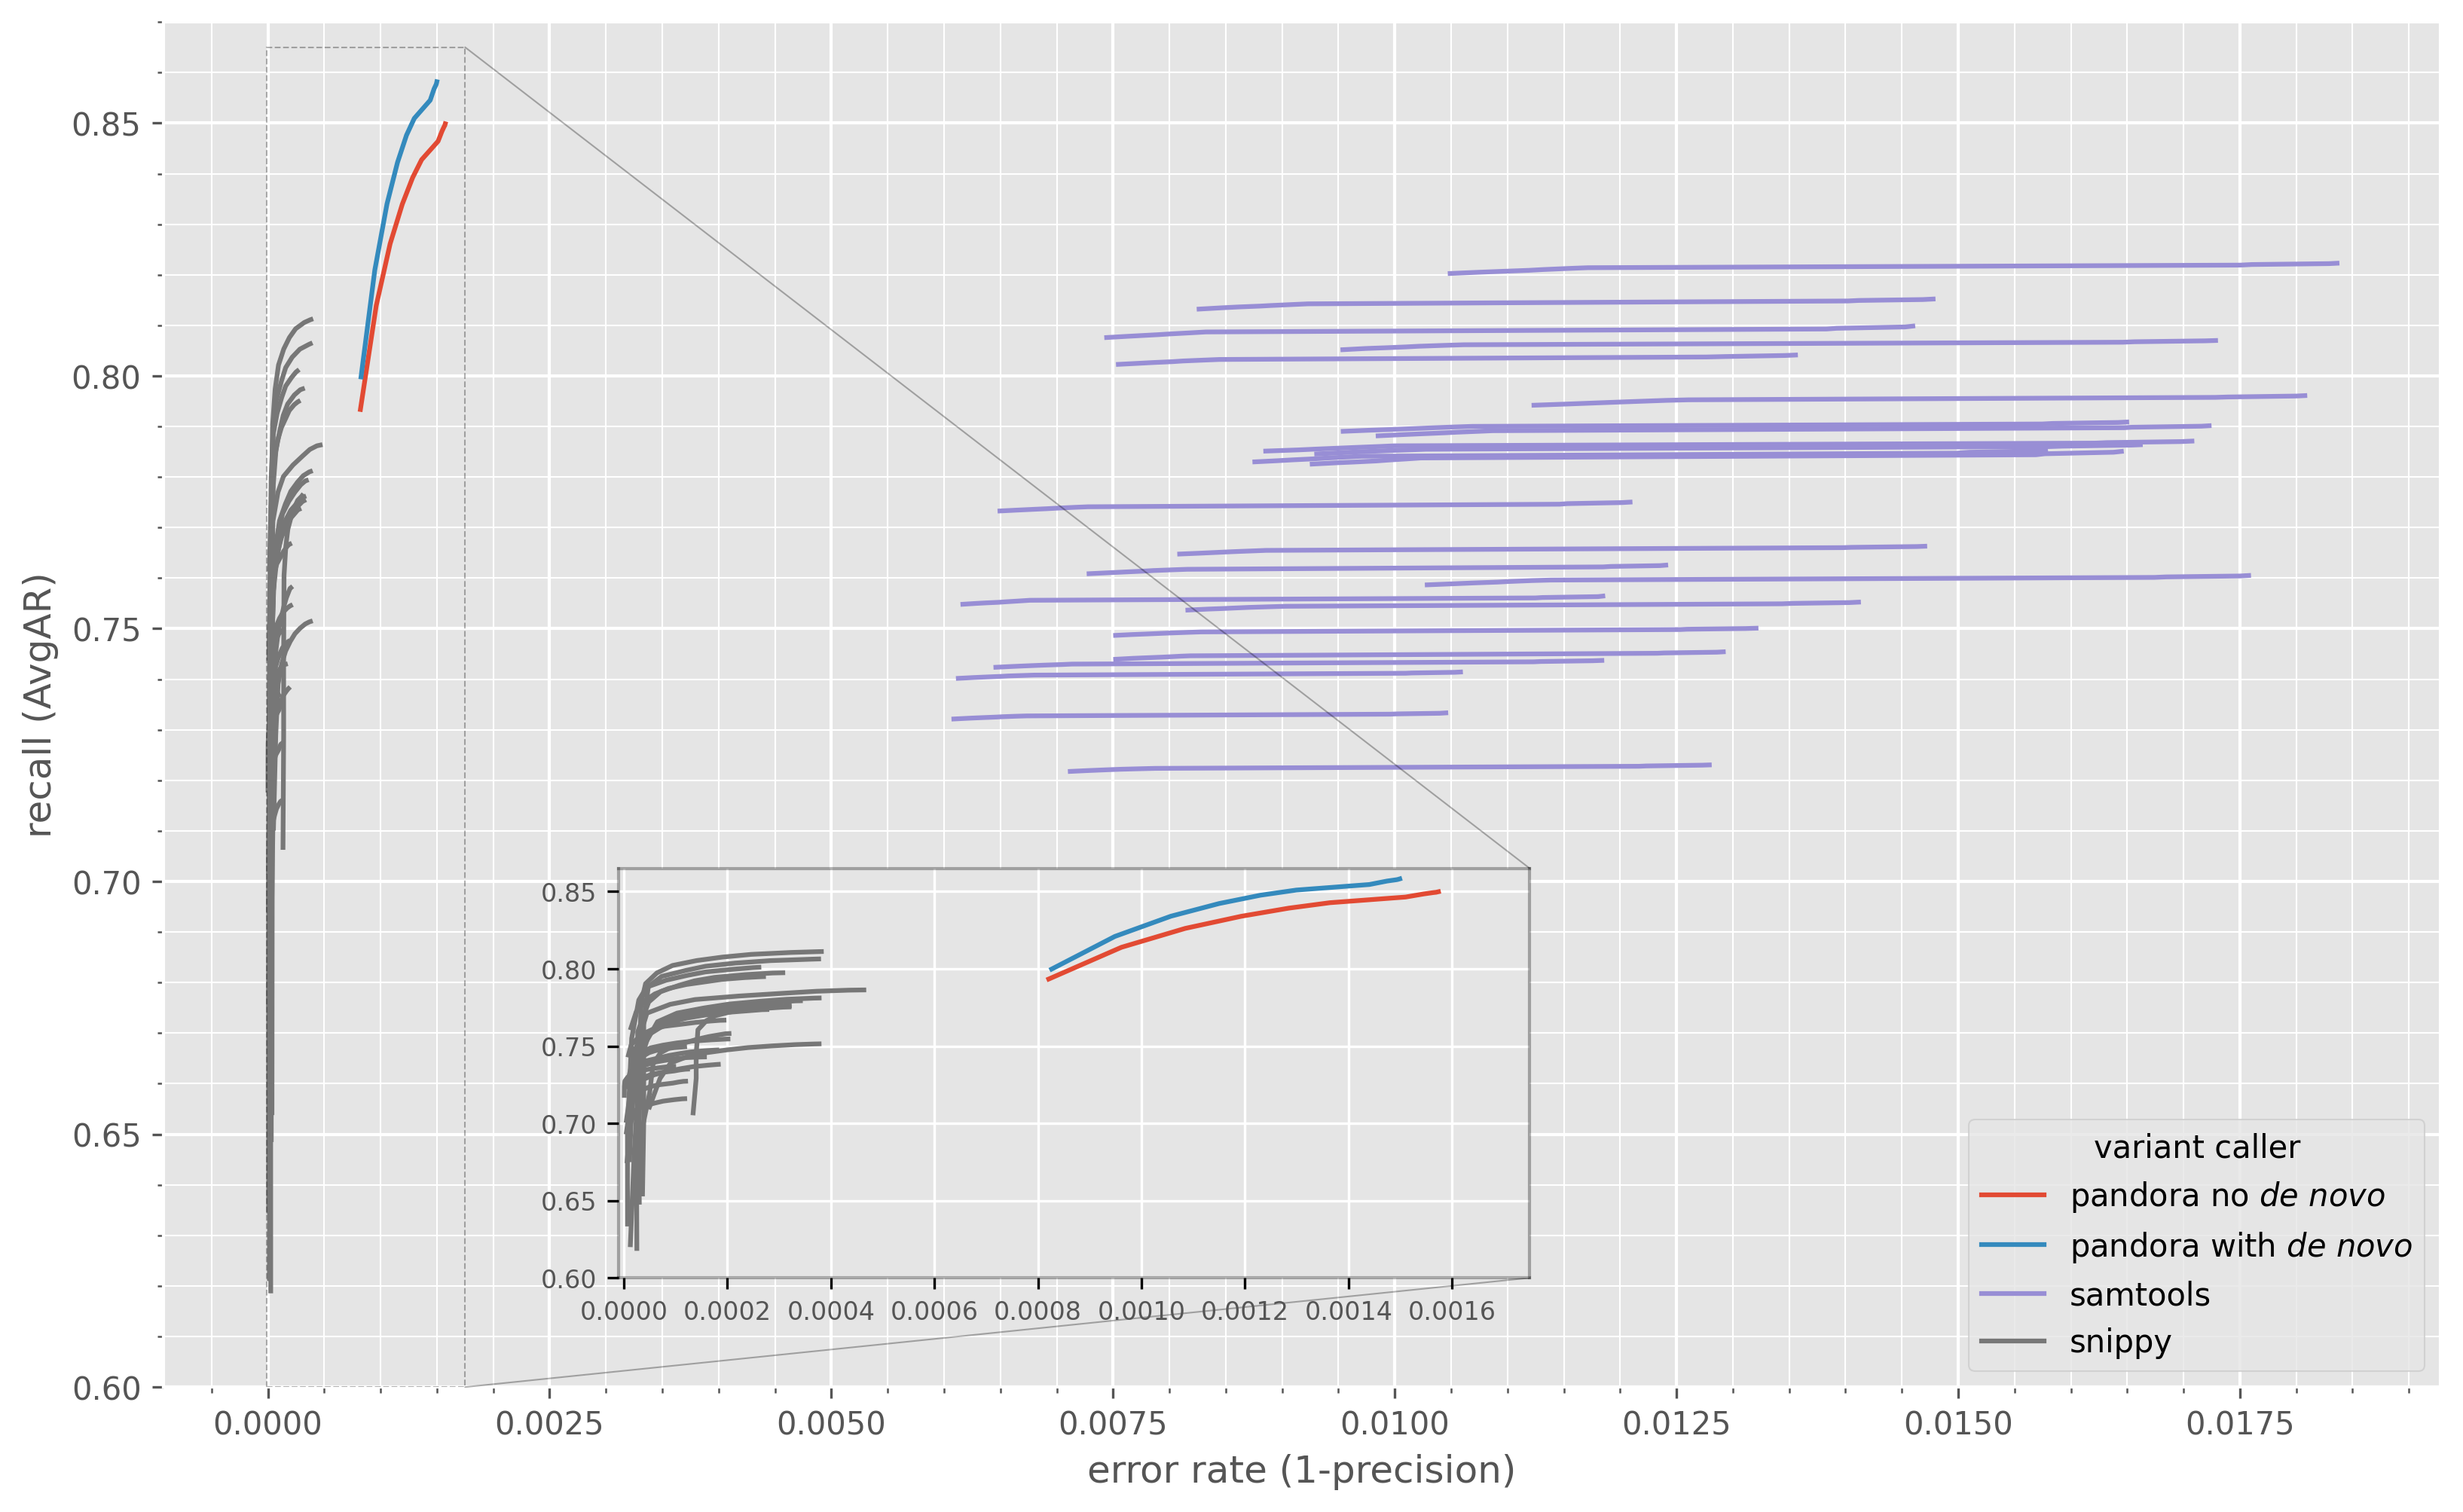
\includegraphics[width=1\linewidth]{Chapter1/Figs/illumina_roc.png}
        \centering
        \caption{Illumina}
        \label{fig:pandora-roc-illumina}
     \end{subfigure}
     \begin{subfigure}[b]{0.475\textwidth}
         \centering
        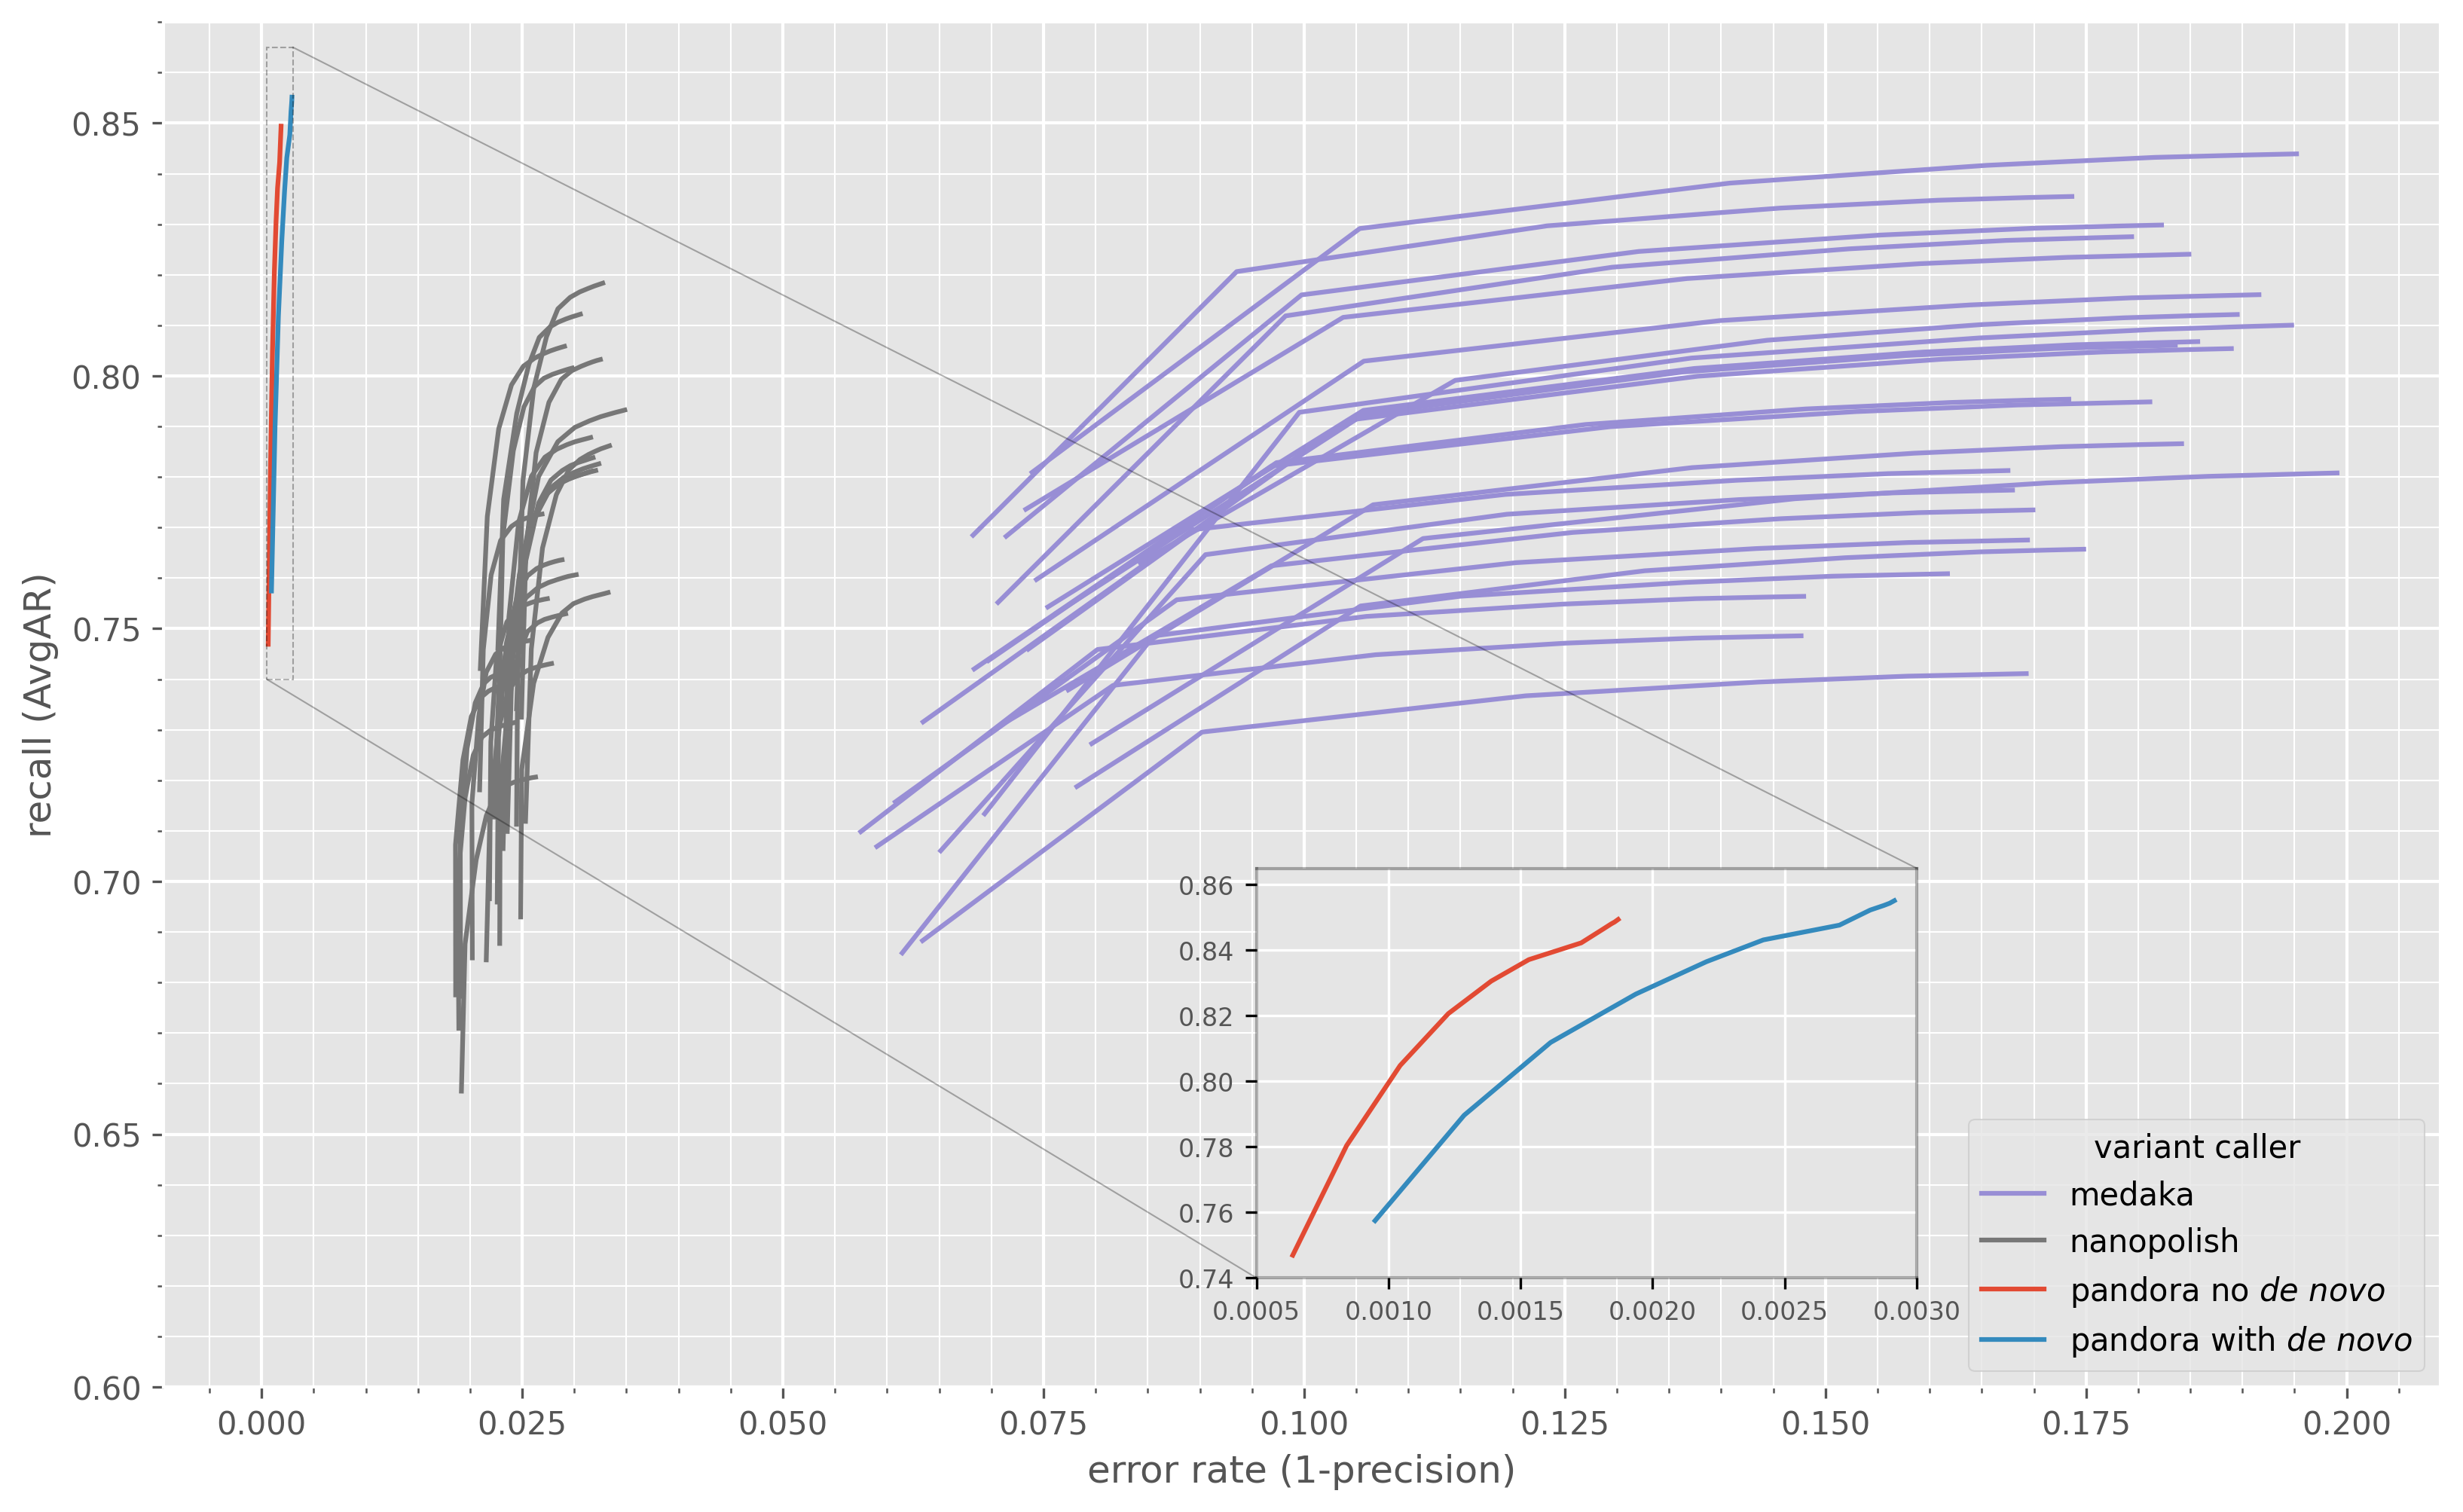
\includegraphics[width=1\linewidth]{Chapter1/Figs/nanopore_roc.png}
         \caption{\ont{}}
         \label{fig:pandora-roc-ont}
     \end{subfigure}
    \caption{Precision-recall curve for variant calls from Illumina (left; \textbf{(a)}) and \ont{} (right; \textbf{(b)}) data for different variant calling tools (colours). Each curve represents increasing genotype confidence thresholds, starting with no filtering in the top-right of each curve and increasing towards the bottom-left. \pandora{} has a single line with (blue) and without (red) \denovo{} variant discovery, which represents the error rate and recall across all 20 samples. The other variant callers are traditional single-reference tools; therefore, each line represents the use of 1/24 reference genomes from across five major \ecoli{} phylogroups. Inset windows are used to give more granularity for error rate in the best performing tools.}
        \label{fig:pandora-roc}
    \source{Adapted from \cite{pandora} under the terms of the \href{https://creativecommons.org/licenses/}{Creative Commons CC BY license}. The colour scheme has been altered, along with the wording of some labels, and the inclusion of inset windows. However, none of these changes in any way alters the underlying data or interpretation of that data.}
\end{figure}

\subsection{Summary}

In this section, using 20 diverse \ecoli{} samples, we have shown that the \denovo{} variant discovery method outlined in \autoref{sec:denovo-method} allows \pandora{} to discover more variants (increases recall). In addition, it improves the error rate on Illumina data.

We also demonstrated that a methylation-aware \ont{} basecalling model decreases the \pandora{} error rate - quite significantly for \denovo{} - indicating that many of the novel variants "discovered" by our method are, in fact, systematic technology errors.

Finally, we show that \pandora{} provides higher recall than single-reference-based variant callers for both Illumina and \ont{} data and leads to a \ont{} error rate that is an order of magnitude lower than other tools. However, \vrb{snippy} provides lower error rates than \pandora{} on Illumina data.

% ==================================================================
\section{Discussion}
\label{sec:denovo-discussion}

In this chapter, we described a method for discovering \denovo{} variation in a genome graph from both Illumina and \ont{} data. We implemented it in the \vrb{discover} subcommand of the reference graph program \pandora{} and evaluated its utility on both simulated and empirical data. Additionally, we demonstrate an approach for comparing variant calls made from single-reference or graph-based tools independent of genome coordinates.

Before the work in this chapter, \pandora{} was only able to genotype with respect to variation present in a pan-genome reference graph. To allow \pandora{} to discover novel variants, we use a localised form of genome assembly in segments of the graph with low \kmer{} coverage. We first identify candidate regions of the genome where read depth (observed as \kmer{} coverage) drops below a predefined threshold. Next, we slice out the segments of the reads that map to these candidate regions and construct a de Bruijn graph from them. Finally, we enumerate paths in this de Bruijn graph that pass coverage and insertion size filters and output them as novel candidate alleles. These alleles can then be added into the original \panrg{} to allow for genotyping against these new alleles.

This \denovo{} discovery process, detailed in \autoref{sec:denovo-method}, is somewhat analogous to the method used by GATK's HaplotypeCaller \cite{Poplin2018}. With two noticeable differences. First, GATK determines candidate regions (described as \emph{ActiveRegions}) based on an "activity score" that is calculated from alignment quality and genotype likelihood at a locus. In contrast, we use a naive approach that looks for \kmer{}s in the maximum likelihood path with coverage less than a hard threshold. While our approach may seem simple, it relies on information gained by performing quasi-mapping to the graph and inference of a maximum likelihood path, which is far from simple. Second, the pruning methods employed by GATK involve removing edges with low support, and when the terminal \kmer{} of a path does not match the reference sequence, they attempt to use local alignment to merge it. By comparison, we require a path contain the terminal \kmer{}, thus avoiding local alignment. Additionally, we prune the de Bruijn graph by using depth- and breadth-first search to construct a distance map so that we know whether a given \kmer{} in the de Bruijn graph can reach the terminal \kmer{} within a predefined number of graph walks. In this way, we never get stuck in cycles or produce paths longer than a user-defined insertion size. 

While we did not compare \pandora{} runtime to GATK, given the results in \cite{Poplin2018} and the algorithmic details of their method, we suspect our method leads to much faster runtimes due to the pruning of paths and lack of local alignment.

\noindent
In \autoref{sec:denovo-sims} we selected random paths from a \panrg{} and randomly introduced SNPs to each at varying rates. We then simulated \ont{} reads from these mutated random genomes and used them to test different parameters relating to our \denovo{} discovery method. Read depth (coverage) had the most obvious impact on the ability to detect novel variants. Given the simulated \ont{} read error rate of approximately 11\%, the decrease in recall with coverage is expected as our method relies on \kmer{} coverage along the candidate paths. Without sufficient \kmer{} coverage to support a path, we cannot produce any candidate alleles. While a \kmer{} size of 13 for \denovo{} assembly was found to perform slightly better than 11 and 15, this was only marginal and may warrant further investigation. Indeed, for the work in \cite{pandora} we used a \denovo{} \kmer{} size of 15 in order to speed up variant discovery in some problematic loci.

While we compared the precision and recall of \pandora{} with and without variant discovery in the simulations, this was not a realistic scenario. In reality, positions within a bacterial genome are under differing levels of selection pressure - e.g., sites that correspond to the third codon position are under weaker pressure than those in the first position \cite{Lobry2002}. However, these simulations do serve to illustrate the limitations of \pandora{} without the capacity to discover variation not present in a \panrg{}.  

\noindent
Given the contrived nature of the simulation analysis,  in \autoref{sec:denovo-empirical} we used an empirical dataset of 20 \ecoli{} samples from across four major phylogroups to examine the benefit of \denovo{} variant discovery. In performing this analysis, we devised a novel method for comparing variant-calling precision and recall across tools in a coordinate-agnostic manner. The main benefit of such an approach is the removal of hard reference bias for \pandora{}, which occurs when the reference genome used for variant calling (or mapping) does not contain a locus (see \autoref{fig:reference-bias}). As the pan-genome of \ecoli{} is open, hard reference bias is a problem when comparing cohorts of diverse samples. Indeed, as shown in Figure 7 of \cite{pandora}, \pandora{}'s use of a locus-specific reference that is dynamically selected based on the cohort under study leads to tens of thousands more SNPs being discovered in rare loci (loci in 2-5 genomes) compared to single-reference variant callers.

An important finding from our empirical analysis is the impact of Enterobacteriaceae methylation on \pandora{}'s \ont{} error rate (\autoref{fig:denovo-methylation}). In particular, when using \denovo{} discovery, the \ont{} error rate is 3-fold lower when a methylation-aware basecalling model is utilised. This observation is also confirmed by Wick \etal{} in their work benchmarking \ont{} basecalling methods for Enterobacteriaceae \cite{wick2019}. They saw that the overwhelming error source was in Dcm methylation sites and that these errors could be virtually erased by training a taxon-specific basecalling model. It follows that given the dramatic decrease in \denovo{} errors as a result of using the methylation-aware model, these systematic biases are being captured and incorporated back into the \panrg{} by variant discovery. Therefore, any \ont{} work involving genomes subject to Dcm methylation would be wise to employ methylation-aware basecalling. Other tools such as \vrb{nanopolish} have incorporated error modelling to remove these systematic biases \cite{Loman2015}. However, as \ont{} sequencing evolves at a rapid pace, the constant maintenance required to model these errors can become very laborious. As such, we feel that taxon-specific basecalling models are a more robust solution to these systematic errors (we explore this further in \autoref{chap:tubby}).

Despite the incorporation of some \ont{} systematic errors caused by \denovo{} variant discovery, we did find that for both Illumina and \ont{} it increased the recall of \pandora{} (\autoref{fig:denovo-methylation} and \autoref{fig:pandora-roc}). In addition, we also found that \denovo{} discovery provided lower error rates on Illumina data (\autoref{fig:pandora-roc-illumina}). As the Illumina and \ont{} data for all samples is matched - i.e., from the same DNA extraction - the difference in error rate between \denovo{} and no-\denovo{} must be technology-driven. However, we do note that the \pandora{} error rate for \ont{} was an order of magnitude lower than both \vrb{medaka} and \vrb{nanopolish}.

\noindent
Without the addition of \denovo{} variant discovery, \pandora{}'s recall is higher than all other variant callers tested - although only marginally higher than \vrb{medaka}. This shows the power of genome graphs to provide access to sections of the genome previously unavailable to single-reference methods. Now that we have provided the functionality for \pandora{} to perform novel variant detection, the door is open to access even more of the pan-genome. 

One application that stands to benefit from pan-genome graphs is prospective surveillance of a bacterial population. The \panrg{} used by \pandora{} is a stable reference capable of handling an evolving cohort and can detect if a strain appears with a new locus. For example, the appearance of the $bla_{NDM-1}$ gene - which confers resistance to carbapenem in Gram-negative bacteria - on plasmids \cite{Yong2009,Kumarasamy2010} might have been more readily detected with the use of a \panrg{}. In this circumstance, hard reference bias can become quite dangerous, and methods without this limitation will more quickly detect concerning loci.

% ==================================================================
\section{Limitations and future work}
\label{sec:denovo-limits}

\subsection{Path enumeration}
\label{sec:fw-path-enum}

A fundamental limitation of the \denovo{} variant discovery method outlined in this chapter is the need for anchor \kmer{}s to initiate local assembly and perform path enumeration. While this is not concerning in most locus areas, it becomes problematic near the start and ends of loci (within $2k-1$ positions of the ends). Indeed, we see in \autoref{fig:denovo-errors} that on simulated data, variants that occur near the ends of loci account for a recall loss of 8\%.

One solution for removing this anchor \kmer{} limitation would be to use a unique \kmer{} approach analogous to Kevlar \cite{Standage2019}. Briefly, Kevlar aims to detect \denovo{} variants by looking for unique \kmer{}s in a child, with respect to the parents. Reads containing these "interesting" \kmer{}s are then assembled with an overlap graph, and the resulting contig is aligned to and genotyped against the reference.

Our idea for how the Kevlar method could be adapted to \pandora{} is to identify candidate regions and extract the read pileups for these regions as we currently do (\autoref{sec:denovo-candidate-regions}). Then, for each candidate region, perform the following: i) let $M$ be the set of all minimizer \kmer{}s along the maximum likelihood path in the candidate region; ii) construct a \kmer{} count table $h(k,c)$ from the read pileup of the candidate region, where $k$ is a minimizer \kmer{} not in $M$ (i.e., $k \notin M$) and $c$ is the number of occurrences of $k$ in the pileup; iii) filter out any $k$ with $c$ less than some threshold determined by the number of reads in the pileup, leaving a set of unique minimizer \kmer{}s $N$. We would then construct a de Bruijn graph from only those reads containing \kmer{}s in $N$. The enumeration of paths through this graph would then involve beginning from any one of the \kmer{}s in $N$ - removing the need for anchors - and only keeping those paths that contain a \kmer{} in $N$. One element of this strategy that requires careful thought is how to incorporate paths back into the graph without the anchor \kmer{}s we currently use.

\subsection{Cycle detection}
\label{sec:denovo-cycles}
The primary computational bottleneck we have encountered during \denovo{} variant discovery development is infinite cycles in the de Bruijn graph. As de Bruijn graphs are directed, but not necessarily acyclic, a cycle can occur when a \kmer{} (node) can reach itself by following a path from any of its successor (out) nodes. When multiple such cycles occur within a graph, computational performance suffers. Such cycles can be detected using depth-first search; however, we do not want to disallow them as cycles are not invalid biologically. 

To limit becoming stuck in cycles, we employ pruning heuristics (\autoref{sec:denovo-prune}) that prevent paths from reaching a maximum length or the exploration of paths that will never reach the end anchor \kmer{}. However, if many cycles occur in close succession, even these heuristics do not prevent bottlenecks. Moreover, in some low complexity \prg{}s, we have seen this process take on the order of days for a single candidate region. As such, future work to improve the computational performance would be well-served to investigate additional pruning strategies. 

\subsection{\ont{} homopolymer deletions}
Wick \etal{} found Dcm methylation sites to be the primary source of errors in Enterobacteriaceae, and when these were eliminated with their taxon-specific model, homopolymer deletions became the chief error source \cite{wick2019}. 

While we did not report the number of homopolymer deletions we found, we did discover one as the source of 1/9 false negatives in our best-performing parameter set in the simulations (\autoref{sec:denovo-sims-results}). As mentioned, some methods attempt to remove these errors as part of their model explicitly. One such possibility would be to refuse to perform \denovo{} discovery on candidate regions containing homopolymer sites. However, we feel such an approach is too coarse and explore a potential solution in \autoref{chap:tubby} that entails training a species-specific \ont{} basecalling model.  

\subsection{Inserting novel alleles into the \panrg{}}
\label{denovo-fw-insert}

In \autoref{sec:denovo-insert} we described a somewhat convoluted process for inserting candidate paths found by \denovo{} discovery into a \panrg{}. This insertion approach is another of the main computational bottlenecks we encountered due to the need to perform a multiple sequence alignment. 

Leandro Ishi has been working on a prototype version of \makeprg{} (\url{https://github.com/leoisl/make_prg}) that facilitates much faster insertion of novel variants into a \panrg{}. When building a \prg{}, it additionally produces a customised data structure that acts as a way of remembering how sequences were clustered and collapsed. In addition, a prototype version (0.9.0) of \pandora{} changes the way \denovo{} discovery produces candidate paths. Rather than outputting them as sequences flanked by the maximum likelihood path sequence, it describes them in a custom format similar to VCF, with the addition of information about the \prg{} site the novel variant occurs in. Leandro has then implemented a new routine within \makeprg{} - \vrb{update} - which takes these custom data structures and attempts to add the novel variants directly into the \prg{}, only requiring the relevant sites to be recalculated. 

\subsection{Insertions and deletions}

A limitation we regret is not including indels in the simulations (\autoref{sec:denovo-sims}). Evaluating indels can become quite complex, and we suspect fine-tuning our method to produce high-quality indel calls will require a lot of time and care. On the other hand, simulations are the ideal environment in which to begin this work, as gathering a truth set of indels for empirical data is notoriously tricky. Thus, future work will begin by including indels in these simulations and then moving to well-characterised indel models for empirical data such as \cite{Bush2021}.

% ==================================================================
\section{Availability of data and materials}

The \pandora{} software is available at \url{https://github.com/rmcolq/pandora} under an MIT license. The \denovo{} method described in this chapter is implement in the command \pandora{} \vrb{discover}.

The analysis pipeline for the simulations in \autoref{sec:denovo-sims} is available at \url{https://github.com/mbhall88/pandora_simulations}. The data used for the \panrg{} in these simulations was obtained from \url{https://pangenome.org/Escherichia_coli}, using the script \url{https://github.com/mbhall88/pandora_simulations/blob/master/scripts/setup_panx_data.sh}. The \ont{} reads used in the simulations was downloaded from Nic Loman's blog post \url{http://lab.loman.net/2017/03/09/ultrareads-for-nanopore/}.

All data and materials for the empirical data analysis in \autoref{sec:denovo-empirical} is described in \cite{pandora} and the corresponding GitHub repository \url{https://github.com/iqbal-lab-org/paper_pandora2020_analyses}.